\thispagestyle{timhieukhoahocnone}
\pagestyle{timhieukhoahoc}
\everymath{\color{timhieukhoahoc}}
\blfootnote{\color{timhieukhoahoc}$^1$Hà Nội.}
\graphicspath{{../timhieukhoahoc/pic/}}
\begingroup
\AddToShipoutPicture*{\put(0,616){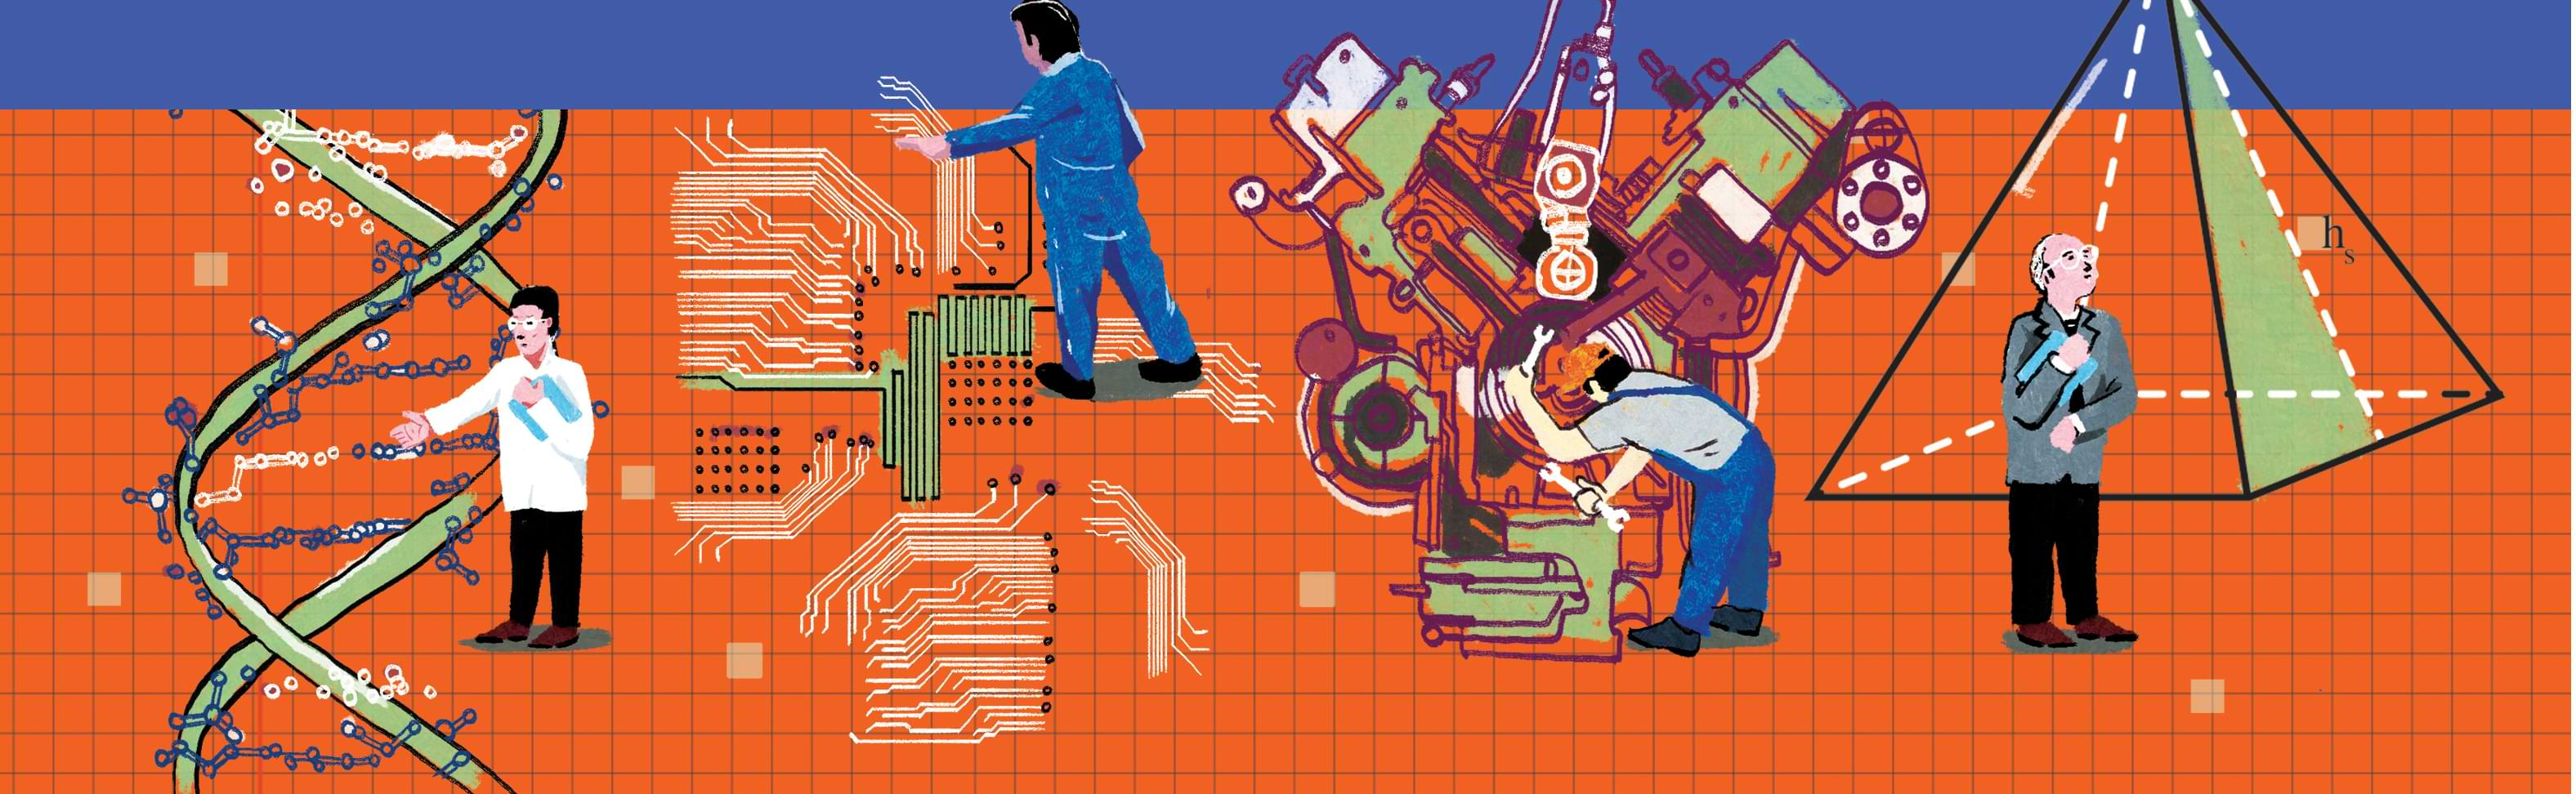
\includegraphics[width=19.3cm]{../bannertimhieu}}}
\AddToShipoutPicture*{\put(144,522){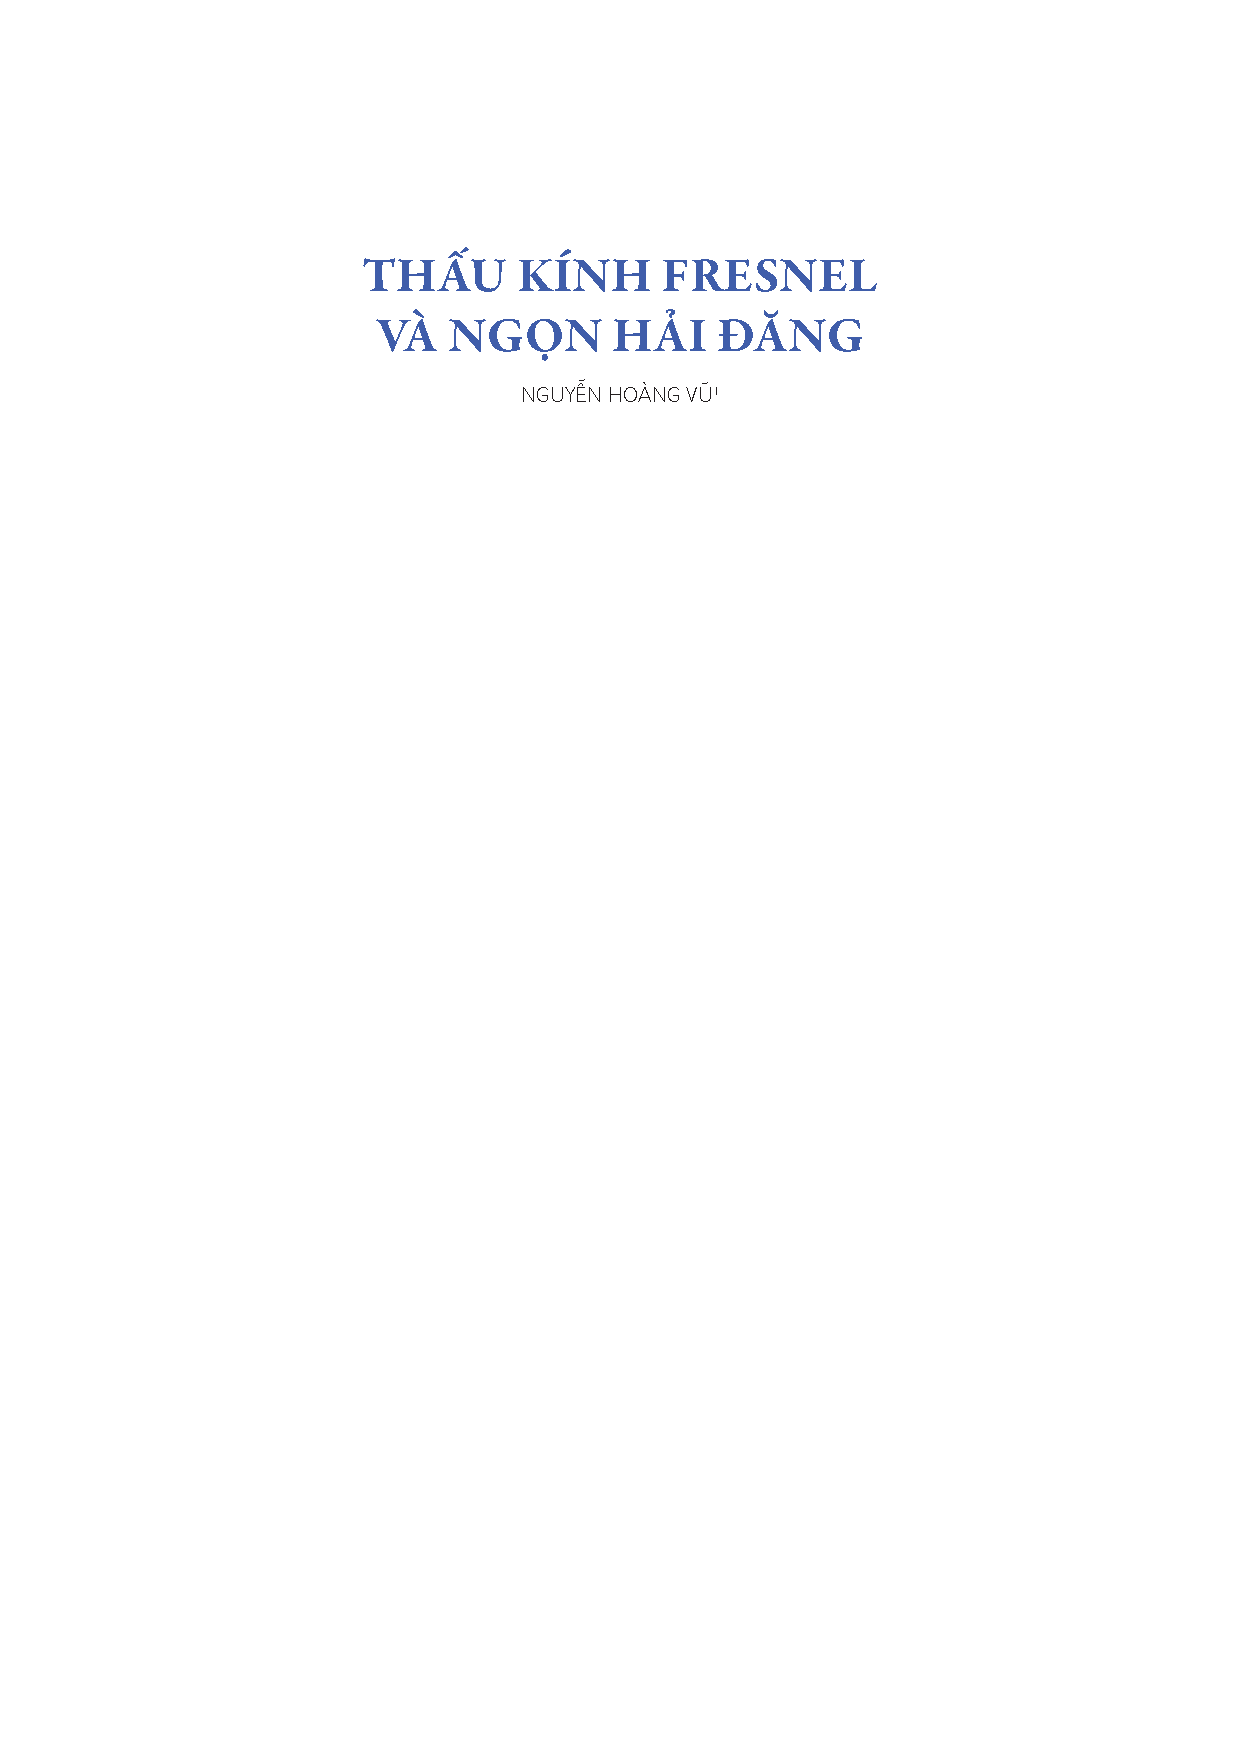
\includegraphics[scale=1]{../tieude1.pdf}}}
\centering
\endgroup
\vspace*{185pt}



\begin{multicols}{2}
	Việc sử dụng ánh sáng để báo hiệu cho tàu thuyền vào gần bờ là một hoạt động hàng hải có lịch sử lâu đời. Tuy nhiên, đến tận đầu thế kỷ $19$, nhiều ngọn hải đăng vẫn hoạt động theo cơ chế như hàng nghìn năm trước đó: nhiên liệu được đốt liên tục trên nóc một tòa nhà cao để ánh sáng tỏa ra không gian xung quanh. Nhiều ngọn hải đăng có lượng tiêu thụ nhiên liệu rất lớn, ví dụ như hải đăng ở Isle of May trên bờ biển Scotland tiêu thụ đến hơn $400$ tấn than đá một năm vào giai đoạn đầu thế kỷ $19$.
	\begin{figure}[H]
		\vspace*{-5pt}
		\centering
		\captionsetup{labelformat= empty, justification=centering}
		
\includegraphics[width= 0.8\linewidth]{1}
		\caption{\small\textit{\color{timhieukhoahoc}Hình $1$. Nhiều ngọn hải đăng cuối thế kỷ $18$ vẫn hoạt động bằng cách đốt than đá tạo thành một đống lửa mà không có hệ thống quang học nào.}}
		\vspace*{-5pt}
	\end{figure}
	\begin{figure}[H]
		\vspace*{5pt}
		\centering
		\captionsetup{labelformat= empty, justification=centering}
		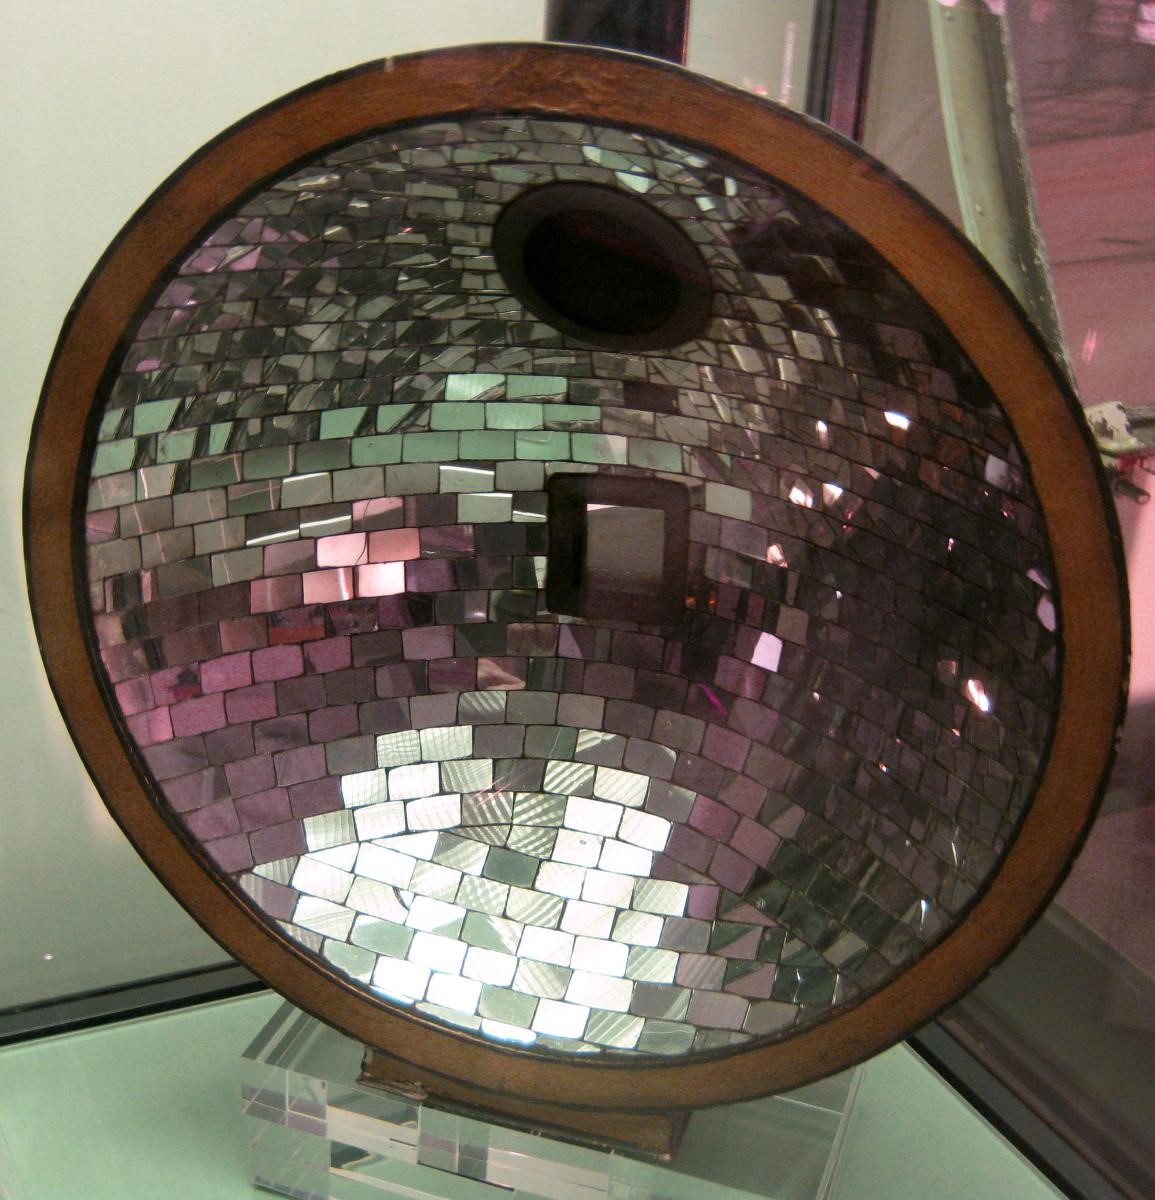
\includegraphics[width= 1\linewidth]{2}
		\caption{\small\textit{\color{timhieukhoahoc}Hình $2$. Mặt phản xạ parabol cho hải đăng của Thomas Smith năm $1787$.}}
		\vspace*{-10pt}
	\end{figure}
	Cũng trong giai đoạn từ cuối thế kỷ $18$ đến đầu thế kỷ $19$, đã có nhiều nỗ lực để cải tiến nguồn sáng của các ngọn hải đăng, một thành phần quan trọng của giao thương hàng hải toàn cầu lúc đó. Một số kỹ sư đã tiến hành sử dụng các mặt phản xạ paraboloid mạ bạc để hội tụ ánh sáng thành chùm song song. Đồng thời, một loại đèn dầu mới do nhà hóa học Thụy Sĩ Aimé Argand thiết kế, còn gọi là đèn Argand, cũng được đưa vào sử dụng với hiệu suất chiếu sáng tốt hơn và không làm đen các mặt phản xạ như những loại đèn trước đó. Do các mặt paraboloid chỉ hội tụ ánh sáng về một hướng nên các ngọn hải đăng sử dụng công nghệ mới này phải trang bị nhiều nguồn sáng khác nhau để bao phủ hết các hướng. Tuy vậy, độ sáng cũng không đồng đều từ trục chính của mặt phản xạ ra bên cạnh.
	
	Năm $1811$, một ủy ban được thành lập ở Pháp với mục tiêu cải thiện các hệ thống chiếu sáng của hải đăng. Do các biến động về chính trị ở Pháp giai đoạn đầu thế kỷ $19$ cùng tính kiêm nhiệm của các thành viên, không có nhiều đột phá mới xảy ra cho đến khi có sự tham dự của Augustin Fresnel vào năm $1819$.
	\vskip 0.1cm
	$\pmb{1.}$ \textbf{\color{timhieukhoahoc}Augustin Fresnel}
	\vskip 0.1cm
	Trước đó, Fresnel đã trở nên nổi tiếng về những nghiên cứu quang học. Các công trình của ông, cũng như của Thomas Young ở Anh, đã chứng minh tính chất sóng của ánh sáng, giống với giả thuyết của Huygens. Fresnel cũng đã phát hiện rằng sóng ánh sáng là sóng ngang, đồng thời giải thích một số hiện tượng quang học như phân cực ánh sáng và khúc xạ kép dựa trên thuyết sóng ánh sáng.
	\begin{figure}[H]
		\vspace*{-5pt}
		\centering
		\captionsetup{labelformat= empty, justification=centering}
		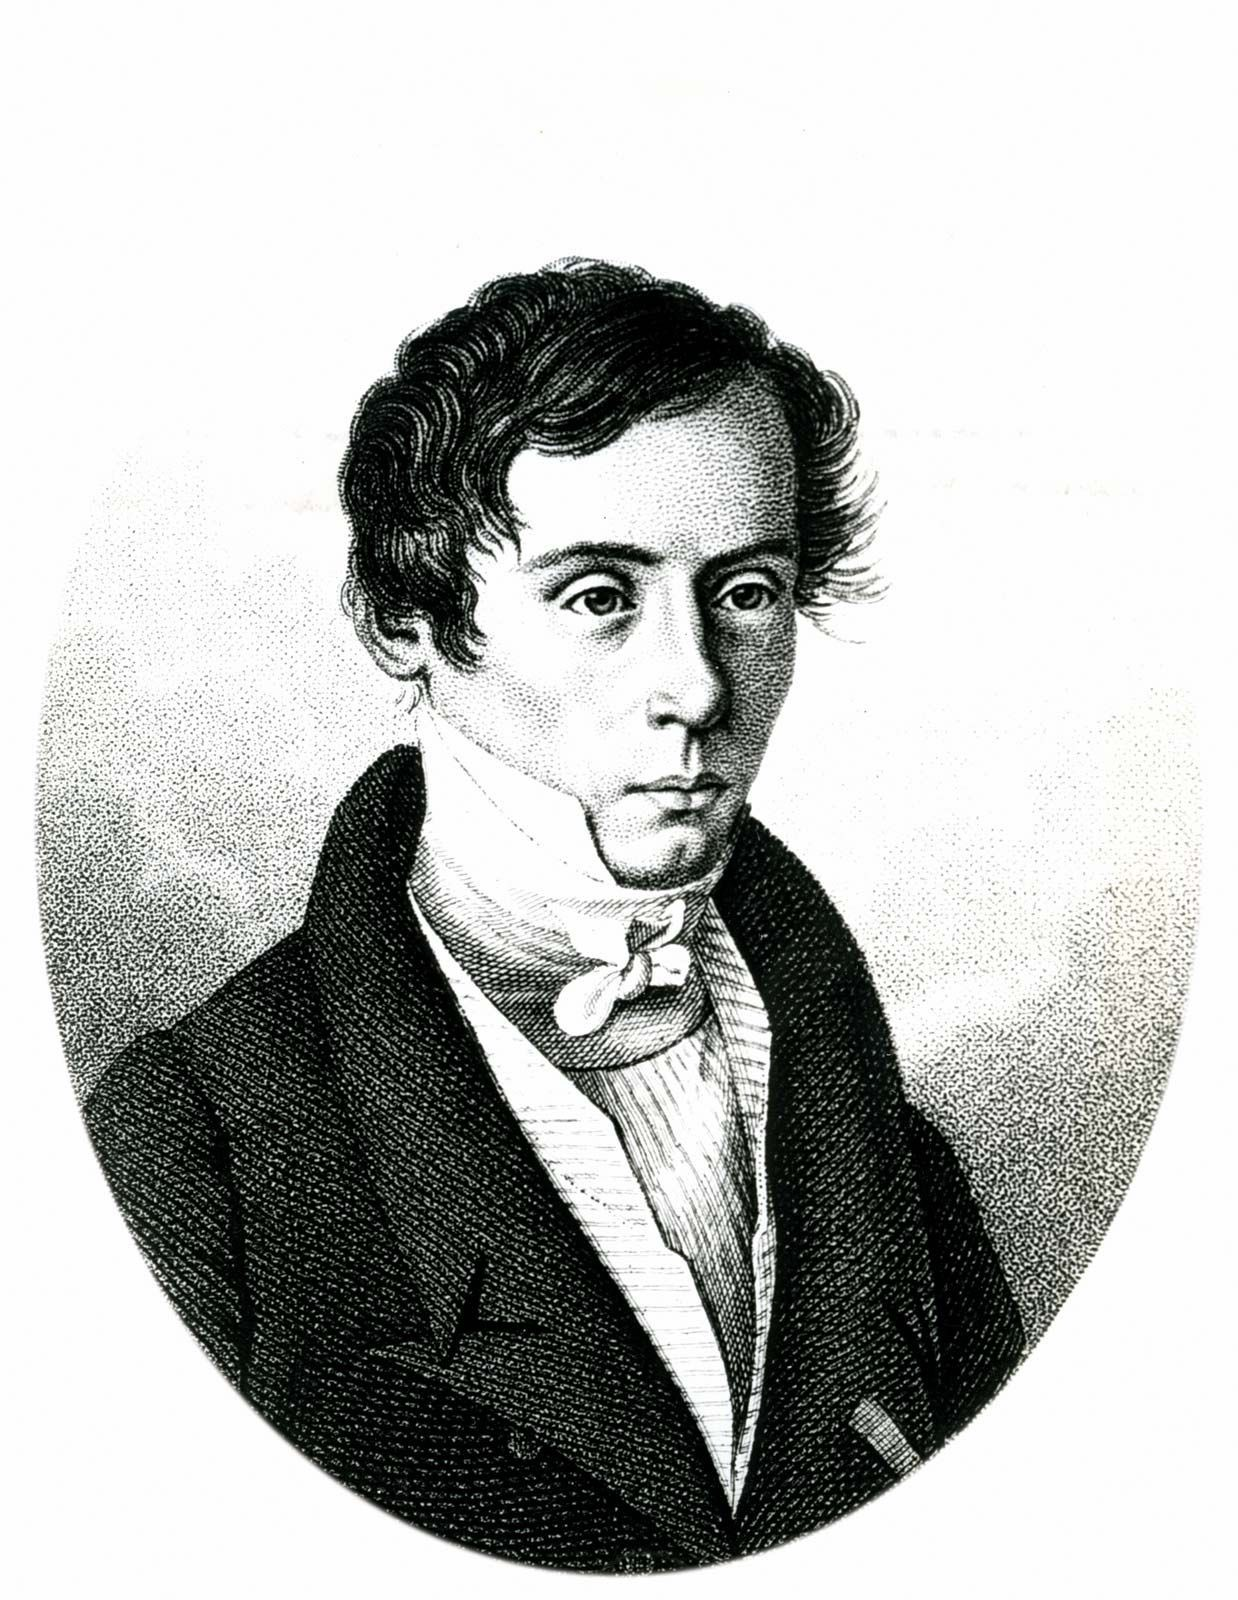
\includegraphics[width= .7\linewidth]{3}
		\caption{\small\textit{\color{timhieukhoahoc}Augustin Fresnel $(1788-1827)$.}}
		\vspace*{-10pt}
	\end{figure}
	Fresnel tham gia vào ủy ban Hải đăng nhờ sự đề cử của Arago, khi đó cũng là thành viên trong ủy ban này. Bản thân Arago cũng là một người ủng hộ nhiệt thành cho thuyết sóng ánh sáng và hai người là cộng sự của nhau trong các nghiên cứu về quang học. Ngay từ khi bắt đầu công việc, Fresnel đã có ý tưởng thay các mặt phản xạ paraboloid bằng các thấu kính do quá trình khúc xạ qua thủy tinh có lượng ánh sáng bị hấp thụ mất ít hơn nhiều so với phản xạ trên các mặt kim loại.
	\vskip 0.1cm
	Tuy nhiên, nếu sử dụng thiết kế thấu kính thủy tinh thông thường, người ta sẽ cần chế tạo một thiết bị quang học có bề dày cũng như khối lượng rất lớn để thỏa mãn yêu cầu quang học cho thiết kế của ngọn hải đăng. Những thử nghiệm trước đó theo hướng này đều đã thất bại. Chỉ trong vòng hai tháng, Fresnel đã cho ra một thiết kế thấu kính mới mà ngày nay được biết đến với tên gọi thấu kính Fresnel để giải quyết vấn đề trên.
	\begin{figure}[H]
		\vspace*{-5pt}
		\centering
		\captionsetup{labelformat= empty, justification=centering}
		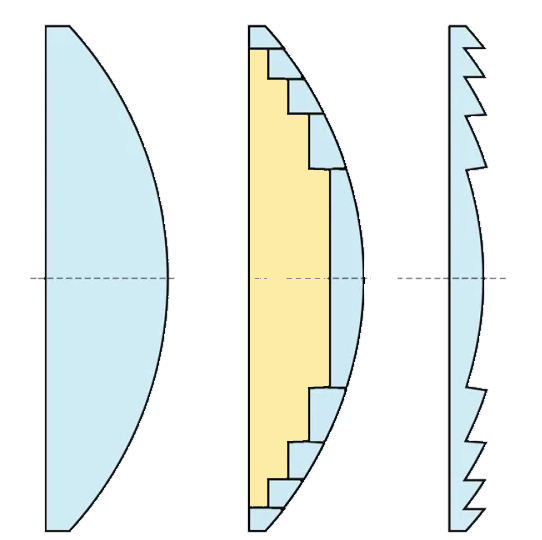
\includegraphics[width= 0.75\linewidth]{4}
		\caption{\small\textit{\color{timhieukhoahoc}Hình $3$. Trái: thấu kính ban đầu. Giữa: Giảm bớt độ dày. Phải: Thấu kính Fresnel gồm các vành tròn đồng tâm.}}
		\vspace*{-10pt}
	\end{figure}
	Thiết kế của thấu kính Fresnel dựa trên một nhận định tương đối đơn giản: trong phần thấu kính  bằng thủy tinh đồng nhất, ánh sáng truyền đi theo đường thẳng. Hiện tượng khúc xạ chỉ xảy ra ở hai mặt của thấu kính tiếp xúc với không khí, là một mặt phẳng và một mặt cong như trong hình. Do đó, nếu ta chia thấu kính ra thành các phần, giảm độ dày giữa hai mặt khúc xạ của mỗi phần và xếp lại, ta được một thấu kính có cấu tạo là các vành tròn ghép lại (Hình $3$). Thấu kính này mỏng hơn nhiều nhưng vẫn cho chùm tia khúc xạ song song nếu mặt cong của mỗi vành được chế tạo theo đúng định luật khúc xạ ánh sáng cho cùng một vị trí tiêu điểm. Nói cách khác, ta được một thấu kính có tiêu cự tương đương thấu kính ban đầu nhưng giảm thiểu đáng kể cả về độ dày lẫn khối lượng. Nhà toán học Buffon cũng đã từng có ý tưởng về một thấu kính tương tự nhưng chỉ với mục đích hội tụ ánh sáng để đốt. Trong khi đó, Fresnel là người đầu tiên sử dụng thấu kính dạng này để tạo chùm sáng song song và tiến hành ứng dụng vào hải đăng. 
	\begin{figure}[H]
		\vspace*{-5pt}
		\centering
		\captionsetup{labelformat= empty, justification=centering}
		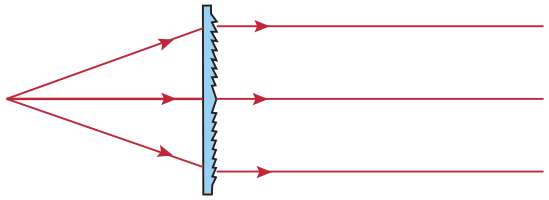
\includegraphics[width= 1\linewidth]{5}
		\caption{\small\textit{\color{timhieukhoahoc}Hình $4$. Thấu kính Fresnel có khả năng biến chùm sáng phát ra từ tiêu điểm thành chùm song song tương tự như thấu kính hội tụ thông thường.}}
		\vspace*{-10pt}
	\end{figure}
	Công việc chế tạo thấu kính Fresnel đầu tiên được tiến hành cùng với François Soleil, một chuyên gia về thiết bị quang học. Một phiên bản thử nghiệm có đường kính $35$ cm được Soleil hoàn thành vào đầu năm $1820$. Các phiên bản lớn hơn ra đời ngay sau đó. Do hạn chế của công nghệ giai đoạn này, với các thấu kính kích cỡ lớn, các vành tròn được thay bằng các vành ghép từ các phần tử quang học dạng đa diện gắn lại với nhau. 
	\vskip 0.1cm
	Sau những thử nghiệm thành công đầu tiên, ủy ban Hải đăng Pháp đã quyết định sử dụng tám khung chứa thấu kính Frensel để lắp đặt tại ngọn hải đăng Cordouan, một trong những ngọn hải đăng nổi tiếng nhất ở trên bờ biển Pháp. Công việc chế tạo lại được thực hiện bởi Soleil. Vào ngày $25$ tháng $7$ năm $1823$, cách ngày nay đúng $200$ năm, hệ thống quang học do Fresnel thiết kế bắt đầu hoạt động ở Cordouan.
	\begin{figure}[H]
		\vspace*{5pt}
		\centering
		\captionsetup{labelformat= empty, justification=centering}
		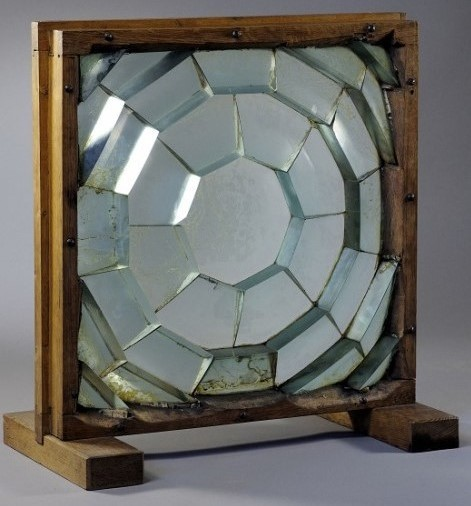
\includegraphics[width= 0.75\linewidth]{6}
		\caption{\small\textit{\color{timhieukhoahoc}Hình $5$. Thấu kính Fresnel thời kì đầu. Do sự hạn chế của công nghệ chế tạo, nhiều khối thủy tinh được ghép với nhau.}}
		\vspace*{-10pt}
	\end{figure}
	Hệ thống này gồm $8$ tấm thẳng đứng tạo thành bát giác đều. Mỗi tấm có một thấu kính Fresnel. Do giới hạn của khúc xạ, chỉ có các tia sáng tạo thành góc nhỏ hơn $45^\circ$ với trục chính đi qua thấu kính. Các tia còn lại sẽ bị thoát ra ở phía trên hoặc phía dưới. Để sử dụng các tia ở phía trên, Fresnel cho lắp đặt các thấu kính Fresnel nghiêng góc nhằm hội tụ chúng thành chùm song song rồi cho phản xạ qua các tấm kim loại để thành chùm song song với phương ngang. Ứng với mỗi cạnh của bát giác sẽ có một tổ hợp thấu kính nghiêng và gương phẳng như vậy. Hệ thống quang học sẽ được quay tròn đều. Với người quan sát, ánh sáng từ ngọn hải đăng sẽ trở nên nhấp nháy theo một tần số nhất định, giúp phân biệt nó với các vì sao hay các nguồn sáng nhân tạo khác (việc sử dụng nguồn sáng biến đổi theo chu kỳ nhờ việc quay đã được áp dụng cho hải đăng từ cuối thế kỷ $18$). Mặt khác, với các tia sáng hướng xuống phía dưới, Fresnel lắp đặt các mặt phản xạ để hướng chúng song song với phương ngang. Tuy nhiên, ánh sáng từ phần này sẽ không quay cùng với hệ thống ở trên và có cường độ cố định. Hệ thống quang học do Fresnel thiết kế cho cường độ ánh sáng quan sát được gấp $8$ lần so với các hệ thống mặt phản xạ dạng paraboloid trước đó, đánh dấu một bước nhảy vọt trong việc đảm bảo an toàn hàng hải. Người ta cũng có thể điều chỉnh để các ngọn hải đăng gần nhau cho ra ánh sáng nhấp nháy với tần số khác nhau. Nếu thủy thủ trên tàu quan sát được cả $2$ ngọn hải đăng cùng lúc, dựa vào bản đồ và góc quan sát tới hai ngọn hải đăng trong thực tế, việc giải bài toán tam giác lượng có thể cho ra vị trí chính xác của tàu.
	\begin{figure}[H]
		\vspace*{-5pt}
		\centering
		\captionsetup{labelformat= empty, justification=centering}
		$a)$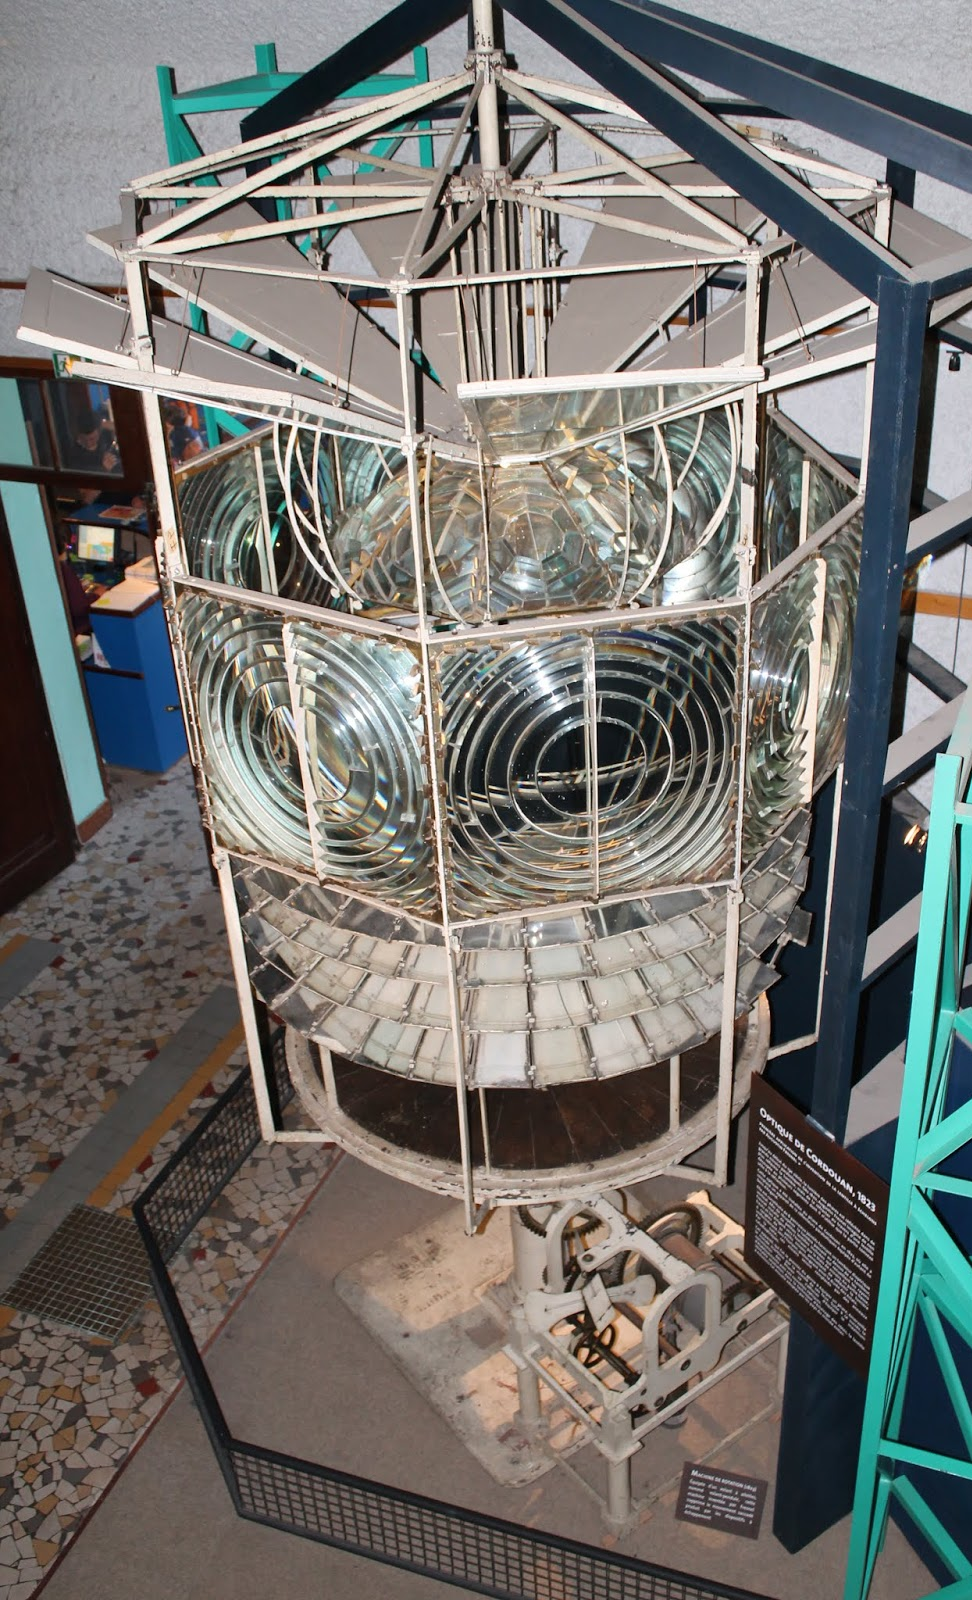
\includegraphics[width= 0.43\linewidth]{7a}
		$b)$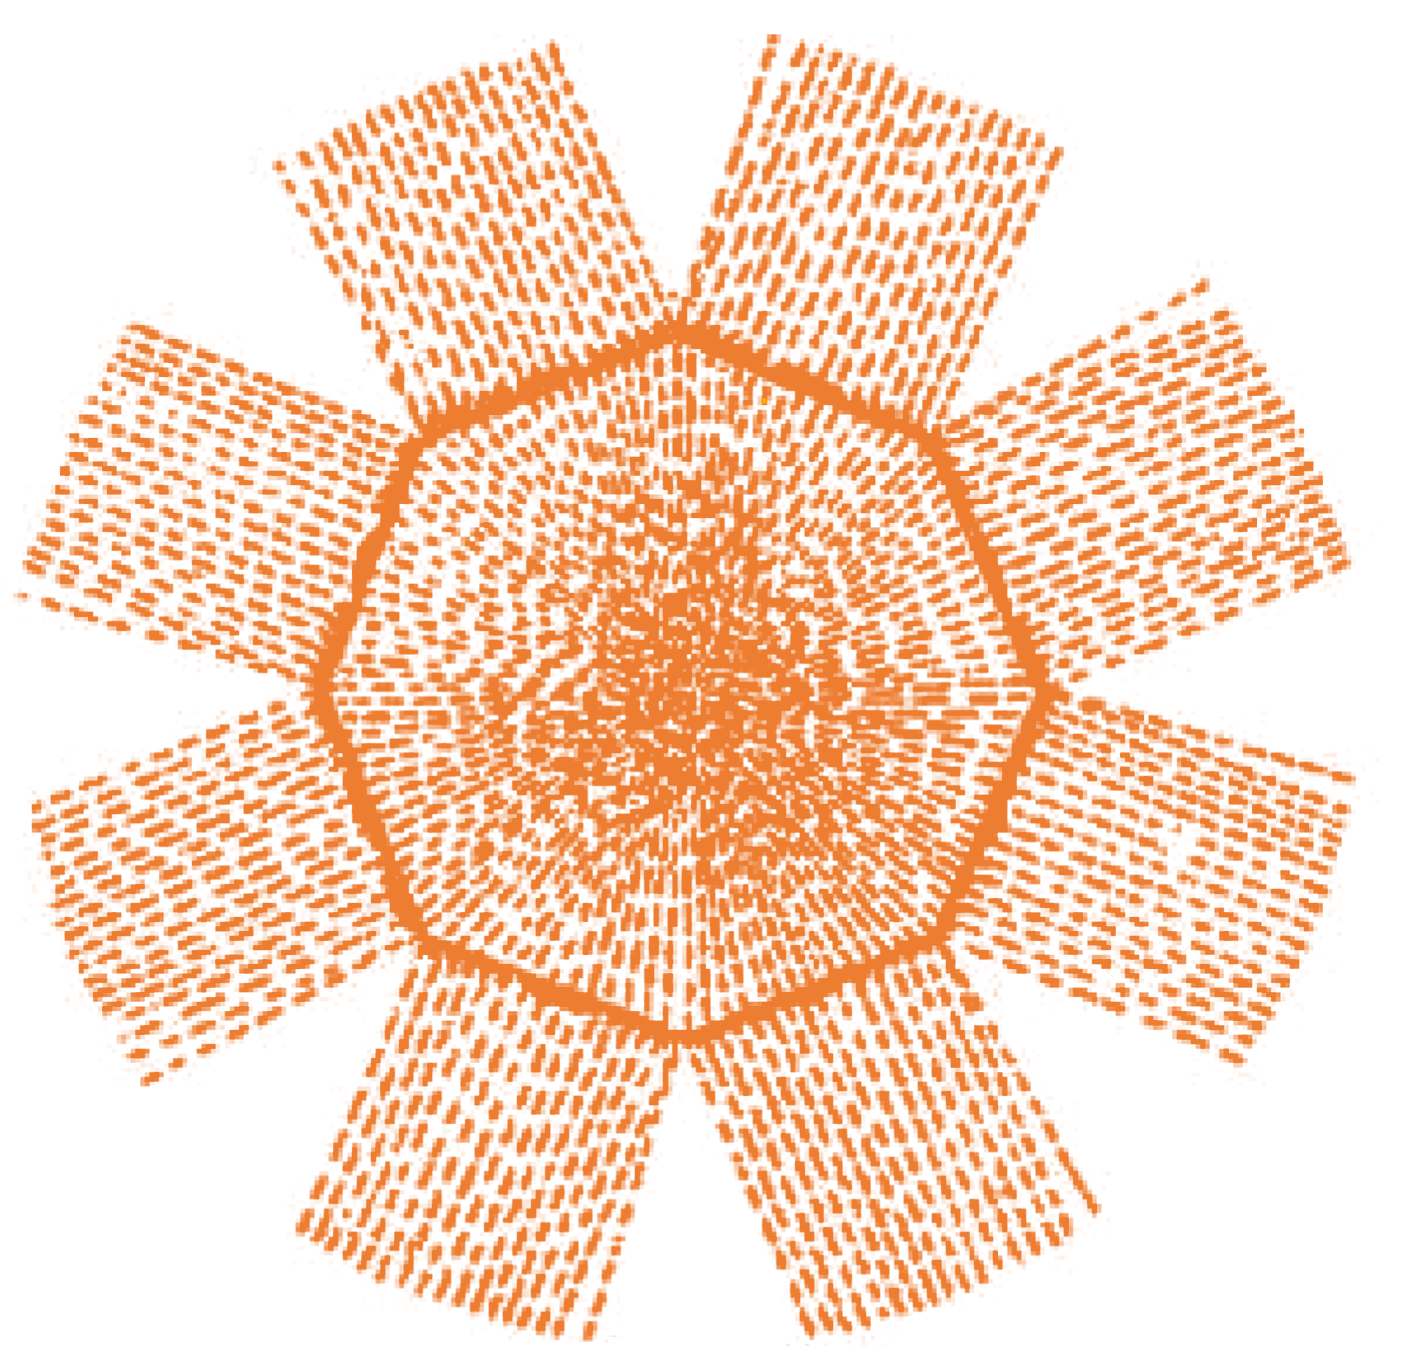
\includegraphics[width= 0.43\linewidth]{7b}
		\caption{\small\textit{\color{timhieukhoahoc}Hình $6$. $a)$ Hệ thống quang học đầu tiên sử dụng thấu kính Fresnel tại Cordouan bao gồm $8$ mặt chứa các thấu kính Fresnel và các hệ thống phản xạ để hứng các tia sáng phía trên và dưới nguồn sáng. $b)$ Khi hệ thống quay, ta thu được $8$ chùm sáng song song mà khi quan sát từ xa sẽ nhấp nháy với tần số cố định.}}
		\vspace*{-10pt}
	\end{figure}
	Trong một số trường hợp khác, người ta chỉ cần ánh sáng cố định -- có cường độ đồng đều theo mọi hướng. Fresnel cũng tiến hành cải tiến thiết kế quang học cho trường hợp này. Toàn bộ phần khúc xạ ở chính giữa là một thấu kính Fresnel dạng tròn xoay với trục quay là trục thẳng đứng để đảm bảo tính đối xứng, do đó ánh sáng sẽ được tán đều theo mọi hướng. Với phần trên và phần dưới, ban đầu Fresnel sử dụng các gương tròn xoay để tạo chùm phản xạ nhưng đến năm $1825$ ông đã có một bước đột phá mới, sử dụng các lăng kính phản xạ toàn phần. 
	\vskip 0.1cm
	Cũng như tên gọi, các lăng kính này hoạt động dựa trên hiện tượng phản xạ toàn phần. Do chiết suất của thủy tinh lớn hơn không khí nên khi tia sáng từ thủy tinh đi ra không khí có góc tới lớn hơn góc tới hạn thì nó sẽ không bị khúc xạ mà toàn bộ tia sáng sẽ bị phản xạ tại mặt tiếp xúc này (Hình $7$).
	\begin{figure}[H]
		\vspace*{-5pt}
		\centering
		\captionsetup{labelformat= empty, justification=centering}
		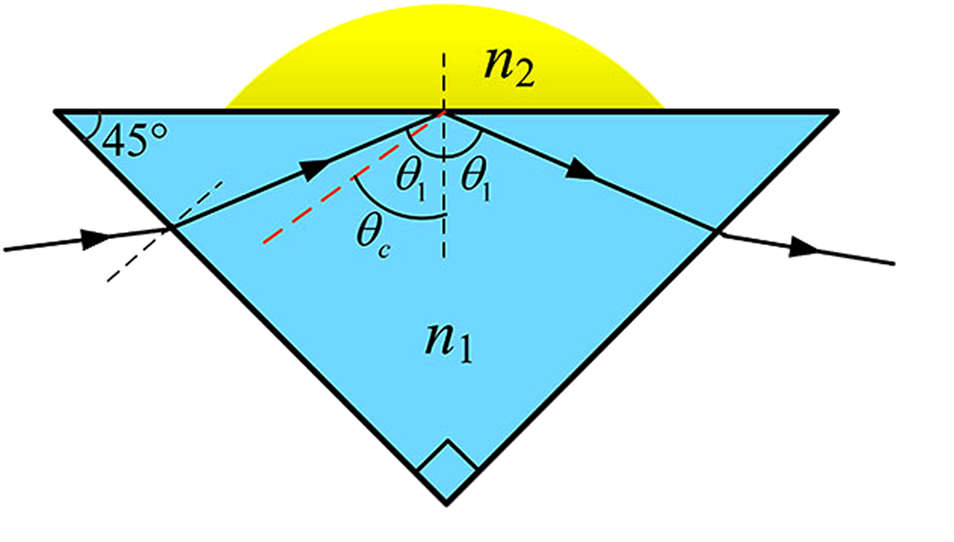
\includegraphics[width= 1\linewidth]{8}
		\caption{\small\textit{\color{timhieukhoahoc}Hình $7$. Lăng kính phản xạ toàn phần. Khi góc tới cạnh huyền lớn hơn góc tới hạn $\theta_c$ với $\sin\theta_c = n_2/n_1$ ($n_1$ và $n_2$ lần lượt là chiết suất của thủy tinh và không khí) thì tia sáng bị phản xạ lại toàn bộ thay vì khúc xạ.}}
		\vspace*{-10pt}
	\end{figure}
	Các lăng kính phản xạ toàn phần tròn xoay (với trục quay là trục thẳng đứng) được Fresnel sử dụng cho phía trên và phía dưới của hệ thống quang học. Thiết kế này đã bổ sung các hạn chế của thấu kính Fresnel, cho ra một hệ thống chiếu sáng đều theo các hướng khác nhau (Hình $8$). Nó cũng đặt cơ sở cho các ý tưởng sau này về việc thiết kế hệ thống quang học hoàn toàn bằng thủy tinh mà không có các mặt kim loại (ánh sáng bị các mặt kim loại hấp thụ khi phản xạ nhiều hơn so với khi khúc xạ hoặc phản xạ toàn phần qua thủy tinh). 
	\begin{figure}[H]
		\vspace*{-5pt}
		\centering
		\captionsetup{labelformat= empty, justification=centering}
		$a)$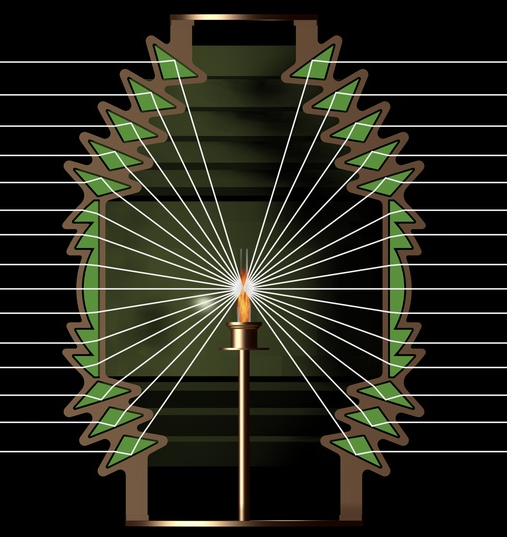
\includegraphics[height=0.53\linewidth]{9}
		$b)$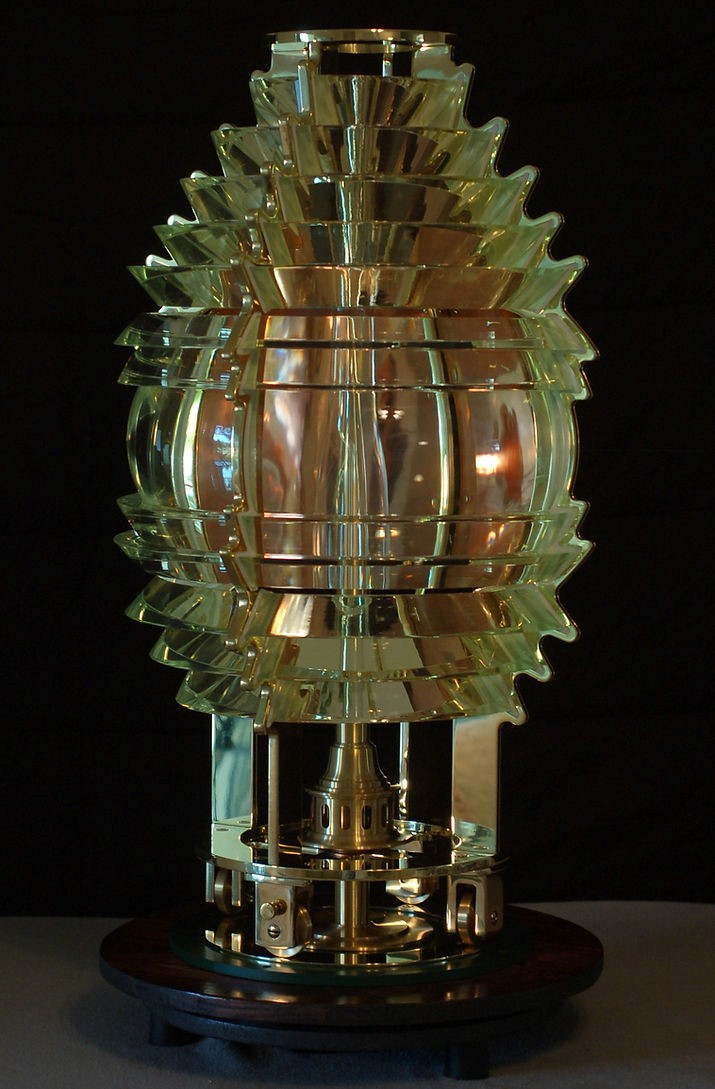
\includegraphics[height=0.53\linewidth]{9b}
		\caption{\small\textit{\color{timhieukhoahoc}Hình $8$. Hệ quang học cho ánh sáng đầu ra cố định. $a)$ Thiết kế sử dụng thấu kính Fresnel và lăng kính phản xạ toàn phẩn. $b)$ Thiết bị trong thực tế gồm các linh kiện là các khối thủy tinh tròn xoay.}}
		\vspace*{-5pt}
	\end{figure}
	Fresnel mất năm $1827$ trước khi thiết kế quang học có lăng kính phản xạ toàn phần được hoàn thiện. Tuy nhiên, ý tưởng này đã được kế thừa và phát triển thêm bởi người em trai Léonor Fresnel cũng như nhiều nhà khoa học và kỹ sư khác của thế kỷ $19$.
	\vskip 0.1cm
	$\pmb{2.}$ \textbf{\color{timhieukhoahoc}Thomas Stevenson và giai đoạn nửa sau thế kỷ $\pmb{19}$}
	\vskip 0.1cm
	Trong giai đoạn sau đó, nhiều cải tiến mới về mặt quang học được tiến hành bởi Thomas Stevenson, con trai của Robert Stevenson, một kỹ sư hải đăng nổi tiếng. Anh trai ông, Alan Stevenson cũng có nhiều cải tiến về thiết kế và chế tạo cho hệ thống quang học của hải đăng dựa trên thấu kính Fresnel. Trong một công bố năm $1850$, Thomas Stevenson đưa ra một thiết kế kết hợp giữa thấu kính Fresnel và mặt phản xạ parabol kim loại (Hình $9$). Các tia sáng đến thấu kính Fresnel được biến thành chùm song song khi nguồn sáng đặt ở tiêu điểm của nó. Các tia sáng chiếu ra phía sau được phản xạ ngược lại nhờ một mặt bán cầu kim loại còn các tia sáng chiếu ra phía trước nhưng không vào thấu kính sẽ được phản xạ nhờ một mặt parabol kim loại có tiêu điểm cũng trùng với vị trí của đèn.
	\begin{figure}[H]
		\vspace*{-5pt}
		\centering
		\captionsetup{labelformat= empty, justification=centering}
		$a)$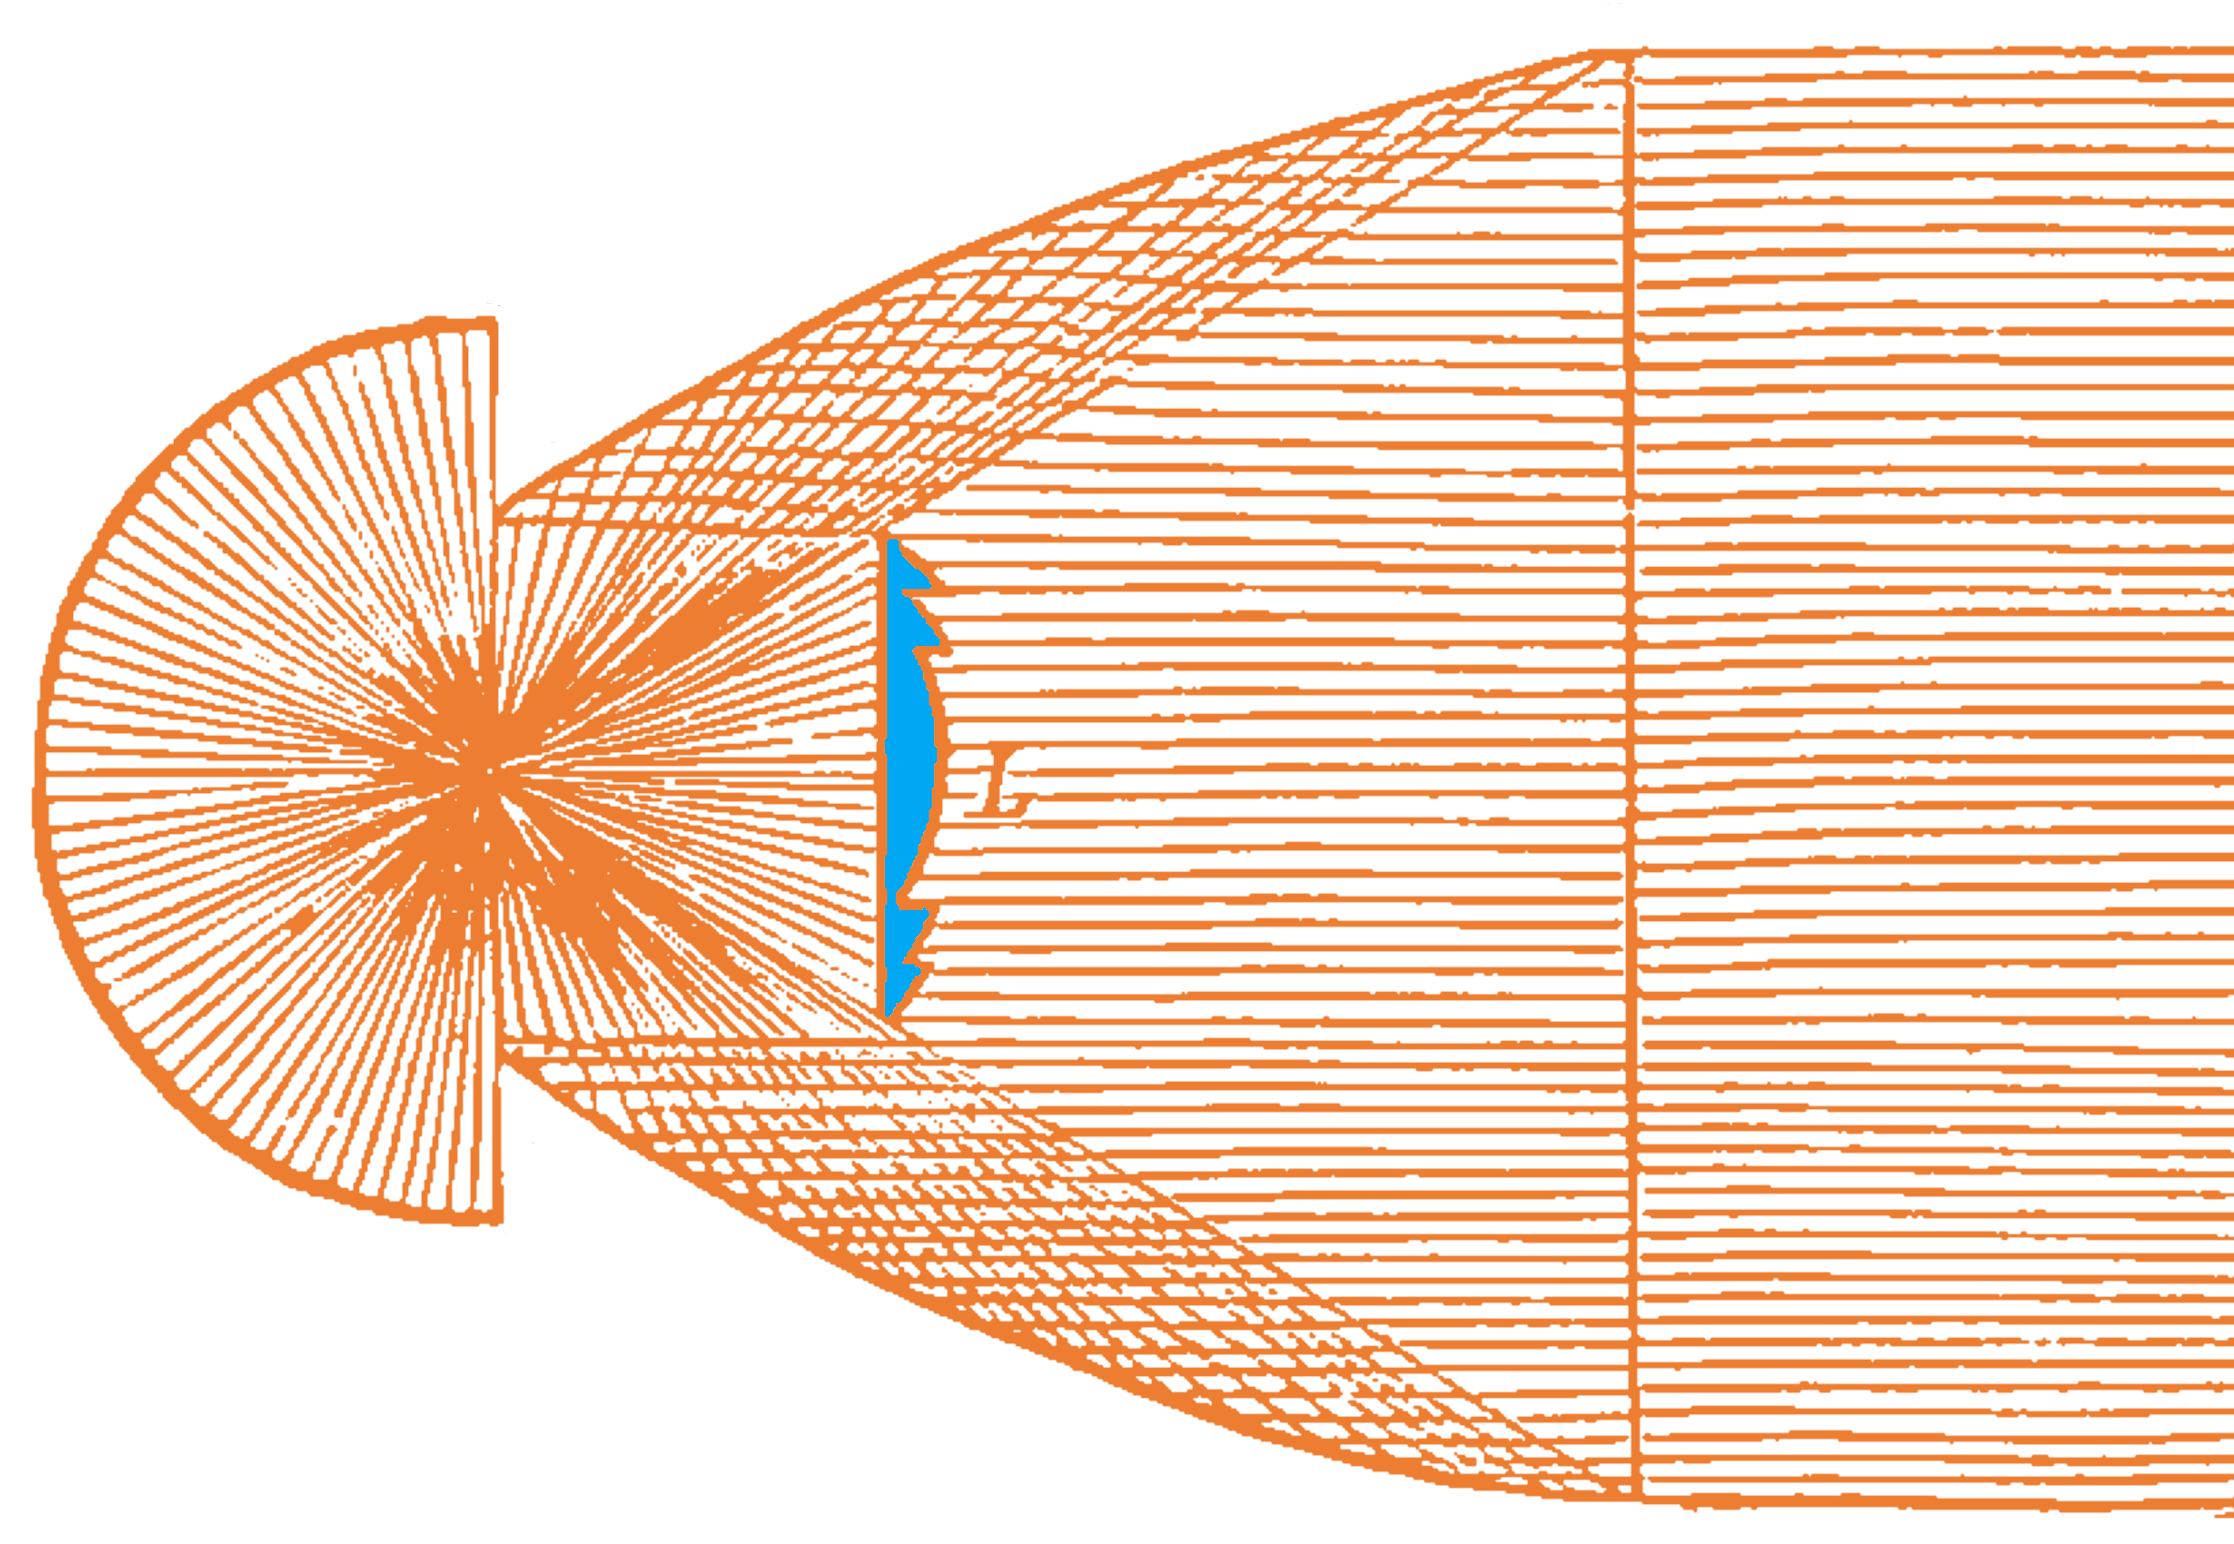
\includegraphics[height= 0.38\linewidth]{10}
		$b)$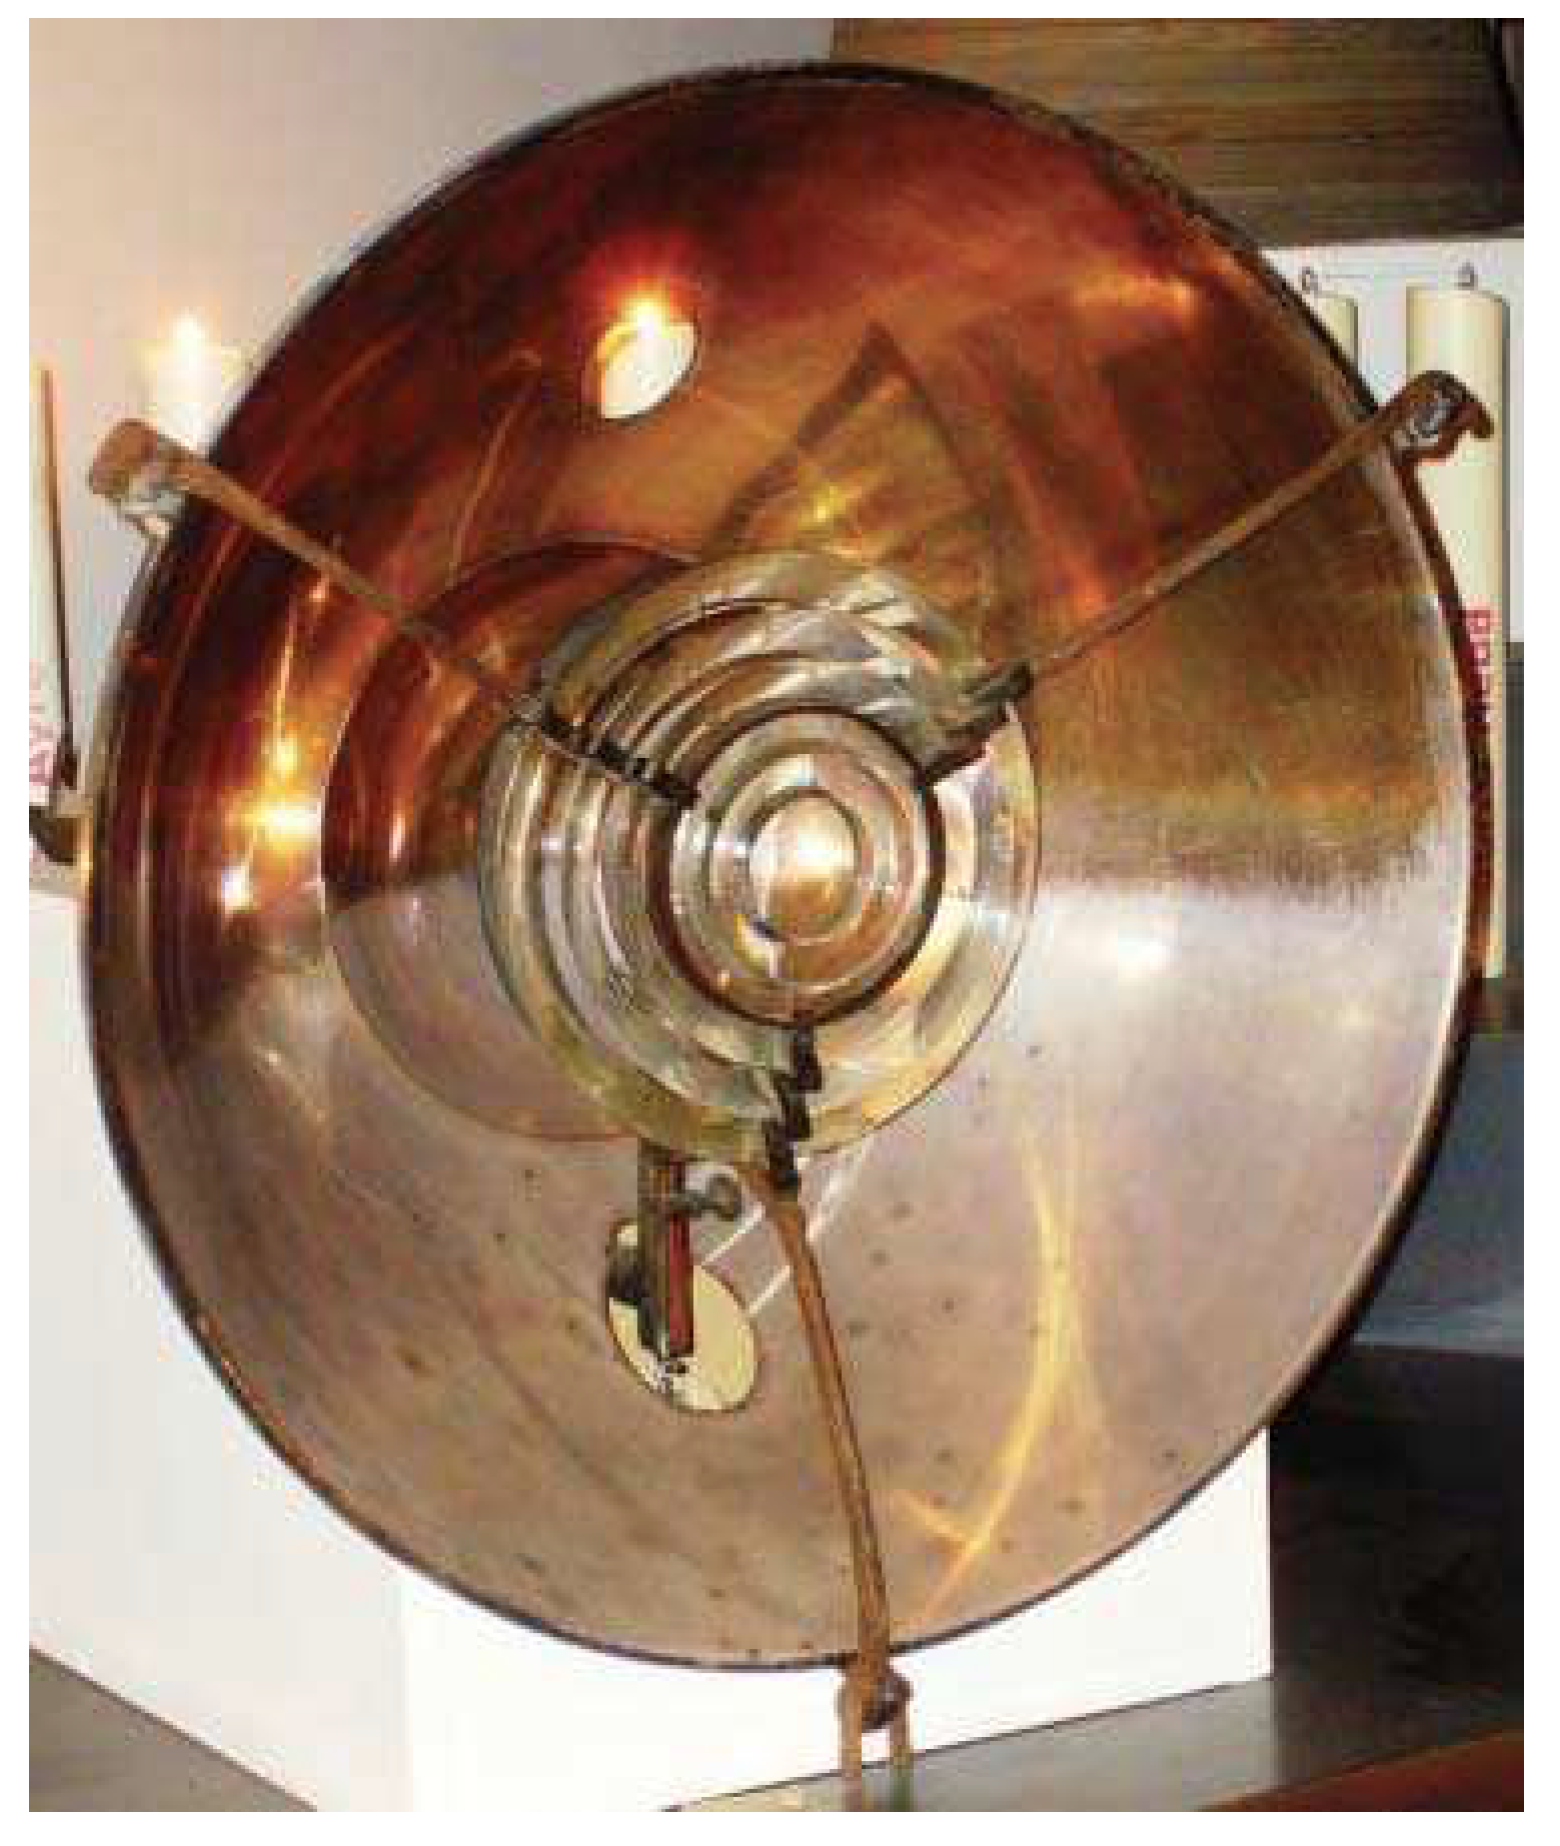
\includegraphics[height= 0.38\linewidth]{10b}
		\caption{\small\textit{\color{timhieukhoahoc}Hình $9$. $a)$ Thiết kế của Stevenson bao gồm một thấu kính Fresnel, một mặt phản xạ parabol và một bán cầu phản xạ bằng kim loại. $b)$ Thiết bị thực tế lắp đặt tại cảng Peterhead.}}
		\vspace*{-10pt}
	\end{figure}
	Stevenson tiếp tục cải tiến bằng cách sử dụng các vành tròn xoay có thiết diện giống với lăng kính phản xạ toàn phần. Điểm khác biệt là trục quay để tạo khối tròn xoay là trục nằm ngang chứ không phải trục thẳng đứng như trong thiết kế của Fresnel. Ông gọi đây là các lăng kính holophote. Chúng có thể được sử dụng để thay thế hoàn toàn mặt parabol kim loại ở phần không gian phía trước nguồn sáng, giúp giảm lượng ánh sáng bị hấp thụ (Hình $10$). Các thiết bị dạng này được lắp đặt tại hải đăng Horsburgh, Singapore năm $1851$.
	\begin{figure}[H]
		\vspace*{-5pt}
		\centering
		\captionsetup{labelformat= empty, justification=centering}
		$a)$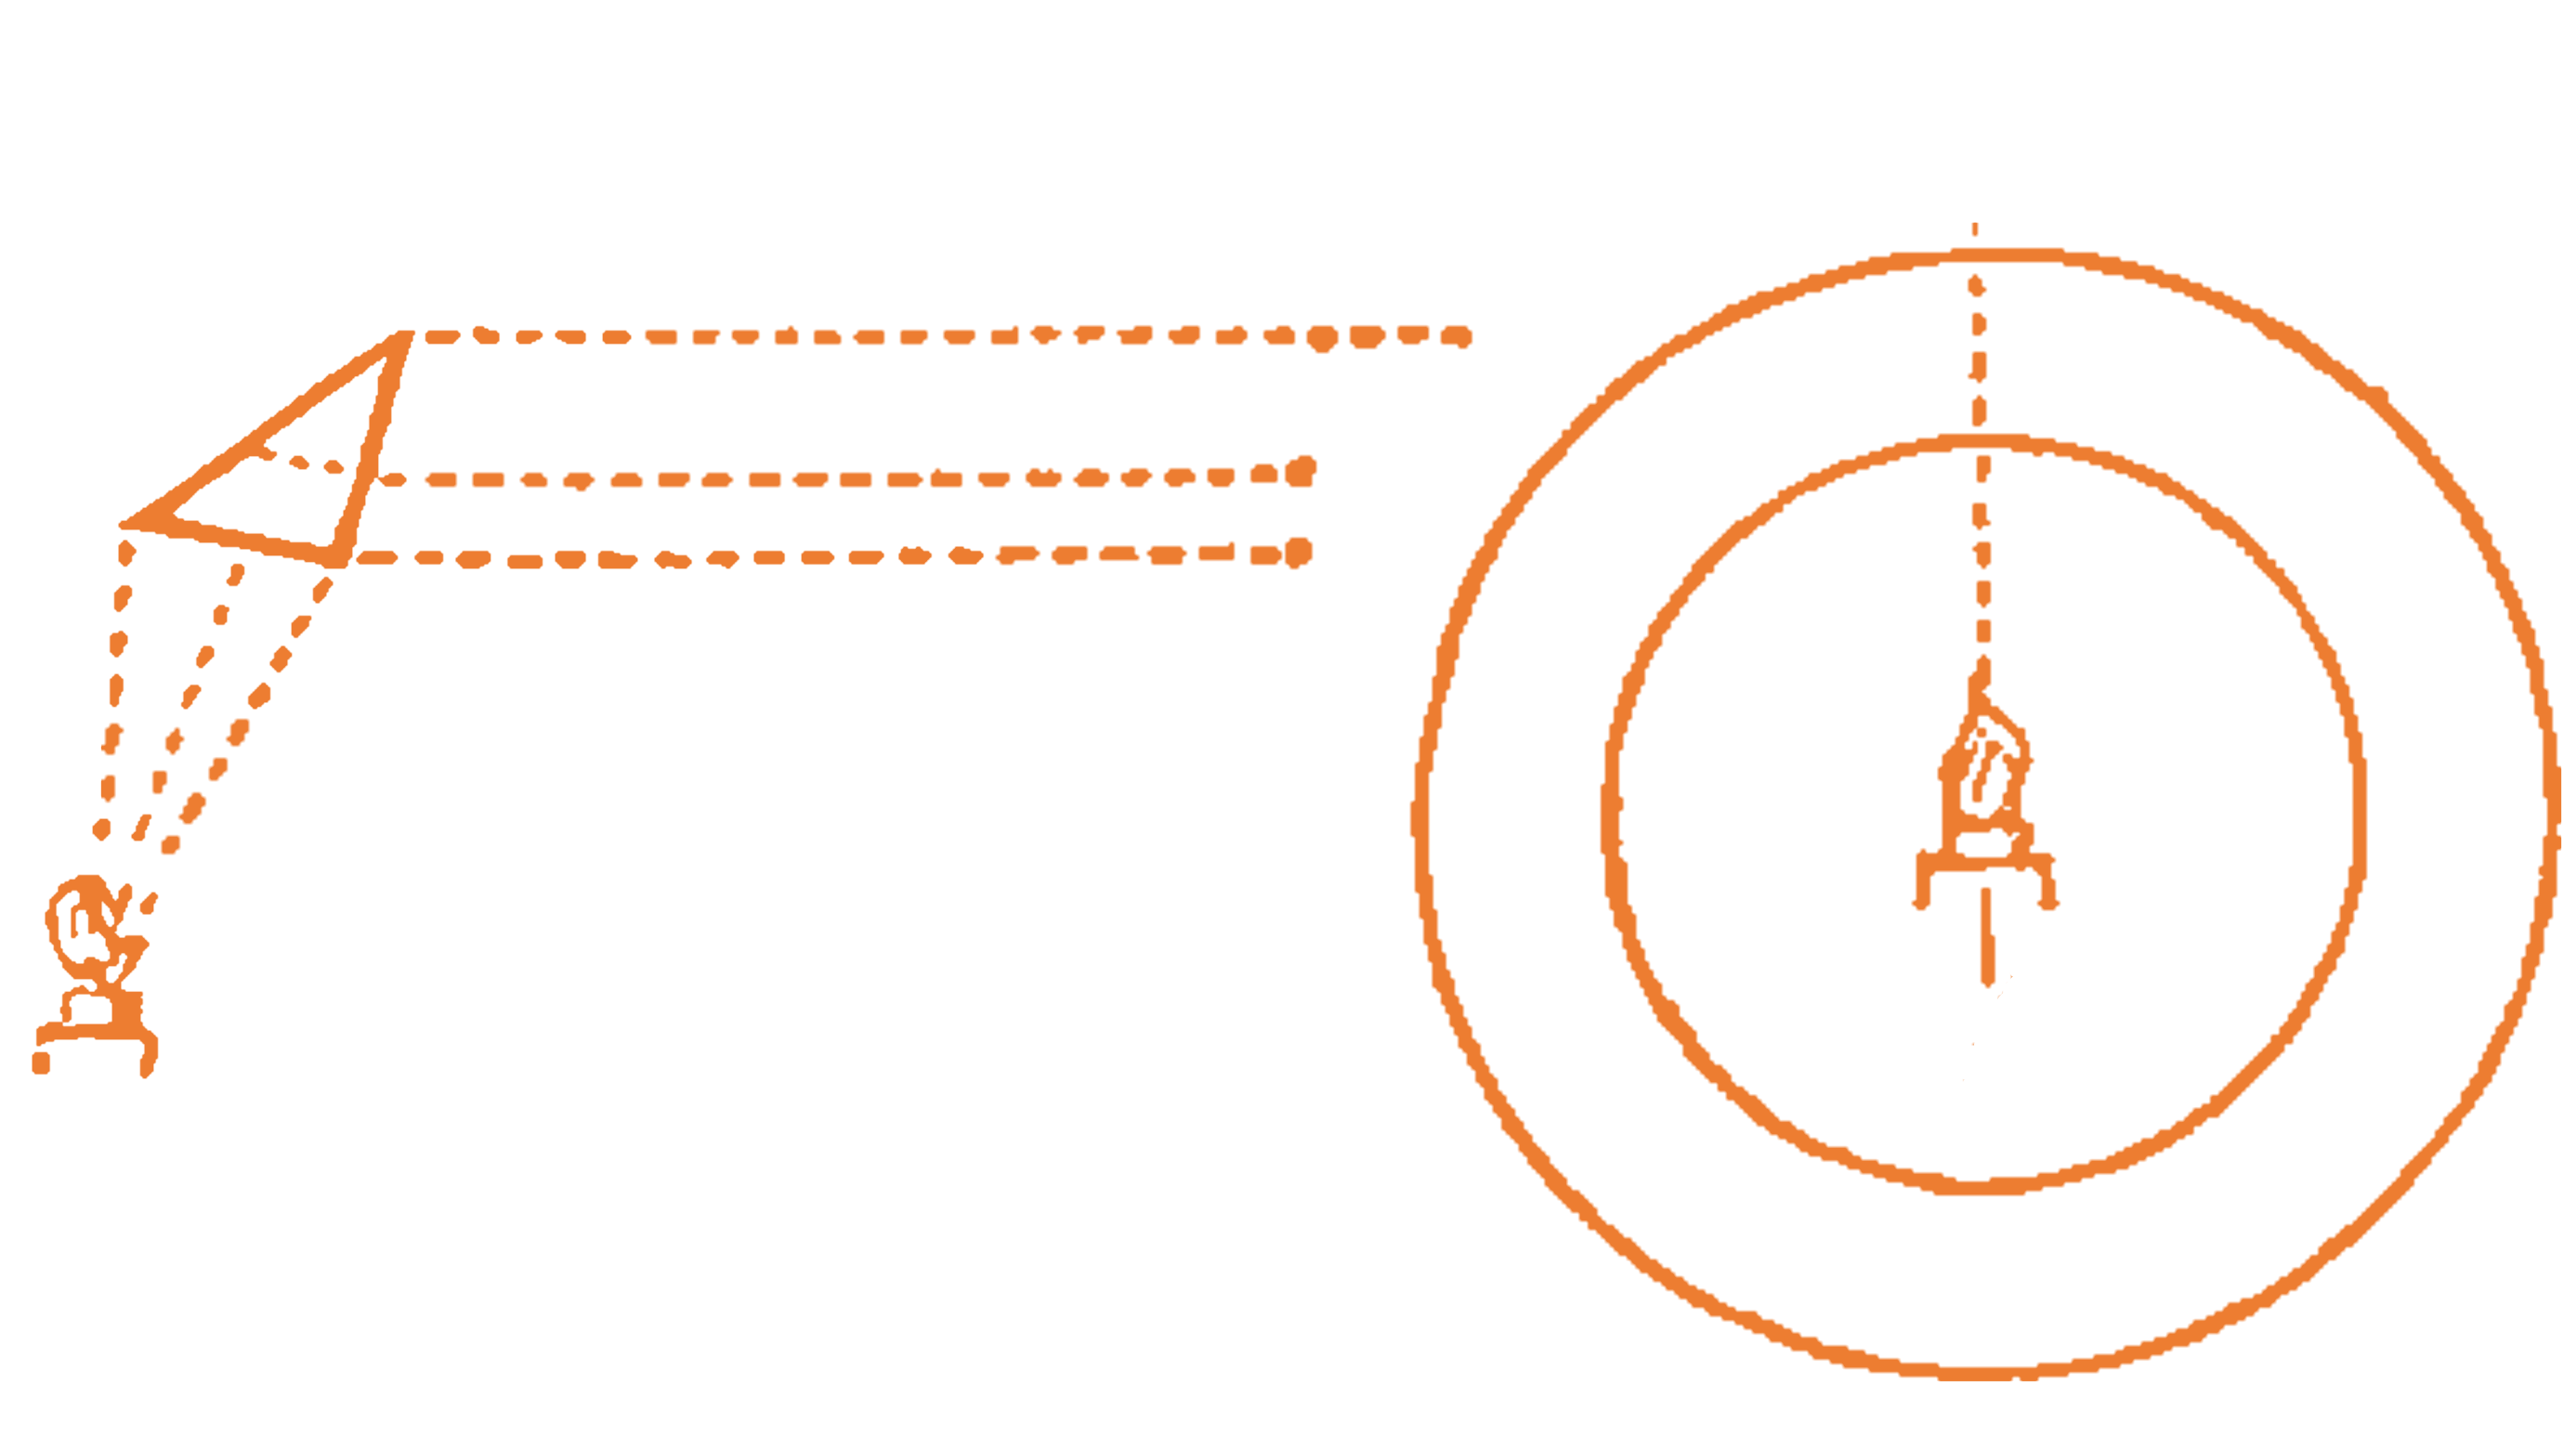
\includegraphics[width= 0.95\linewidth]{11a}
		$b)$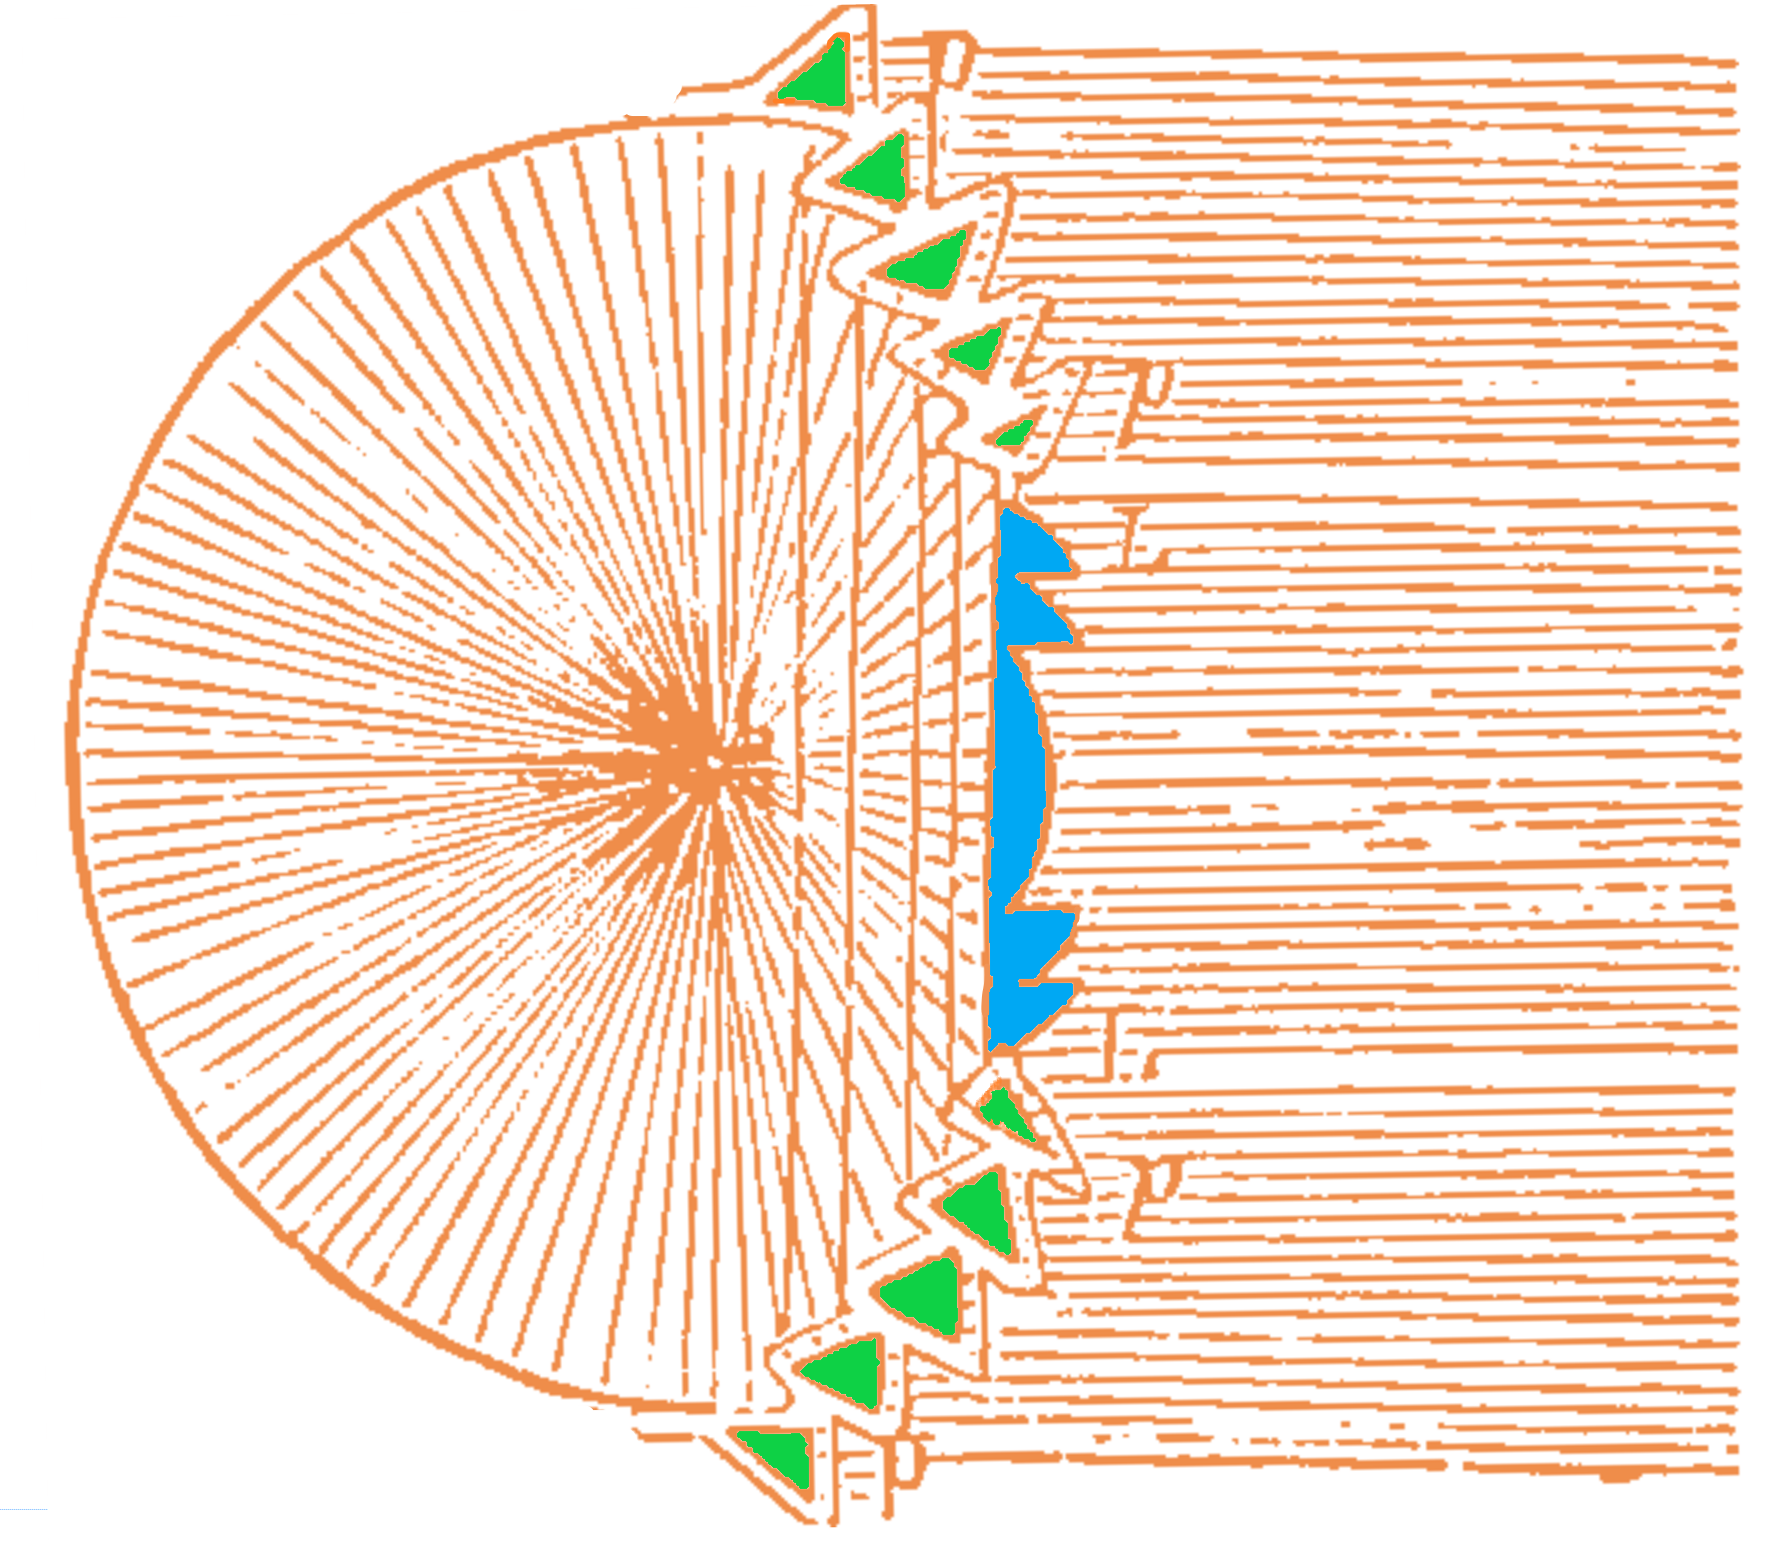
\includegraphics[height= 0.5\linewidth]{11b}
		$c)$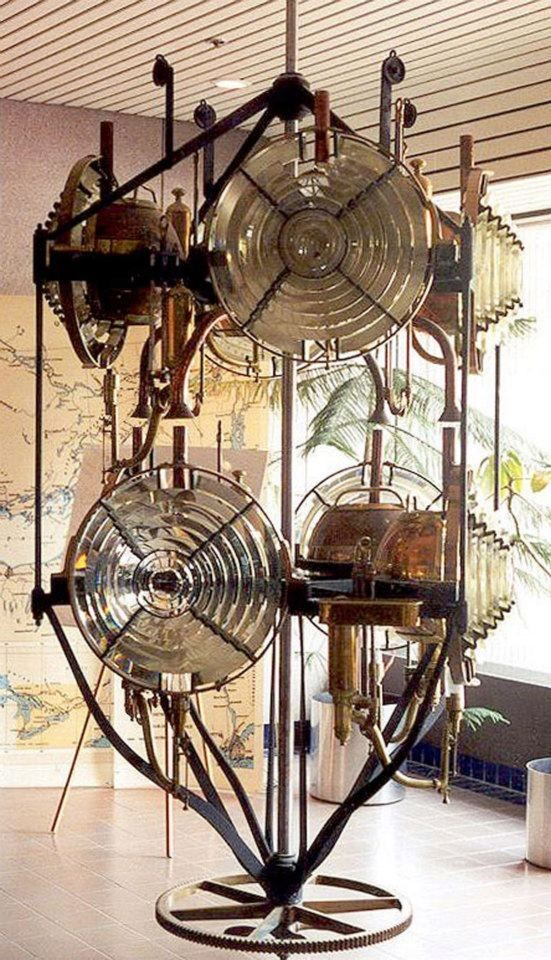
\includegraphics[height= 0.5\linewidth]{11c}
		\caption{\small\textit{\color{timhieukhoahoc}Hình $10$. $a)$ Hình chiếu cạnh và hình chiếu ngang của lăng kính holophote. $b)$ Lăng kính holophote (tô màu xanh lá cây) được sử dung thay cho mặt phản xạ parabol. $c)$ Hiện vật từ thế kỷ $19$. Các lăng kính holophote là các khối tròn xoay xung quanh thấu kính Fresnel ở giữa.}}
		\vspace*{-10pt}
	\end{figure}
	Cuối cùng, để loại trừ vật liệu kim loại cho bán cầu mặt sau nguồn sáng, Stevenson sử dụng một loại lăng kính mới, ngày nay được biết đến với tên gọi lăng kính phản xạ kép. Lăng kính này làm cho tia sáng tại một vị trí cố định bị phản xạ toàn phần hai lần rồi quay lại đúng vị trí ban đầu. Nếu tiến hành kết hợp các lăng kính dạng này, ta có một thành phần quang học hoàn toàn bằng thủy tinh có thể thay thế cho mặt phản xạ dạng bán cầu (Hình $11$). Thiết kế của Stevenson sau đó được James Timmins Chance cải tiến bằng cách sử dụng lăng kính là khối tròn xoay quanh trục thẳng đứng thay vì trục nằm ngang.
	\begin{figure}[H]
		\vspace*{-5pt}
		\centering
		\captionsetup{labelformat= empty, justification=centering}
		$a)$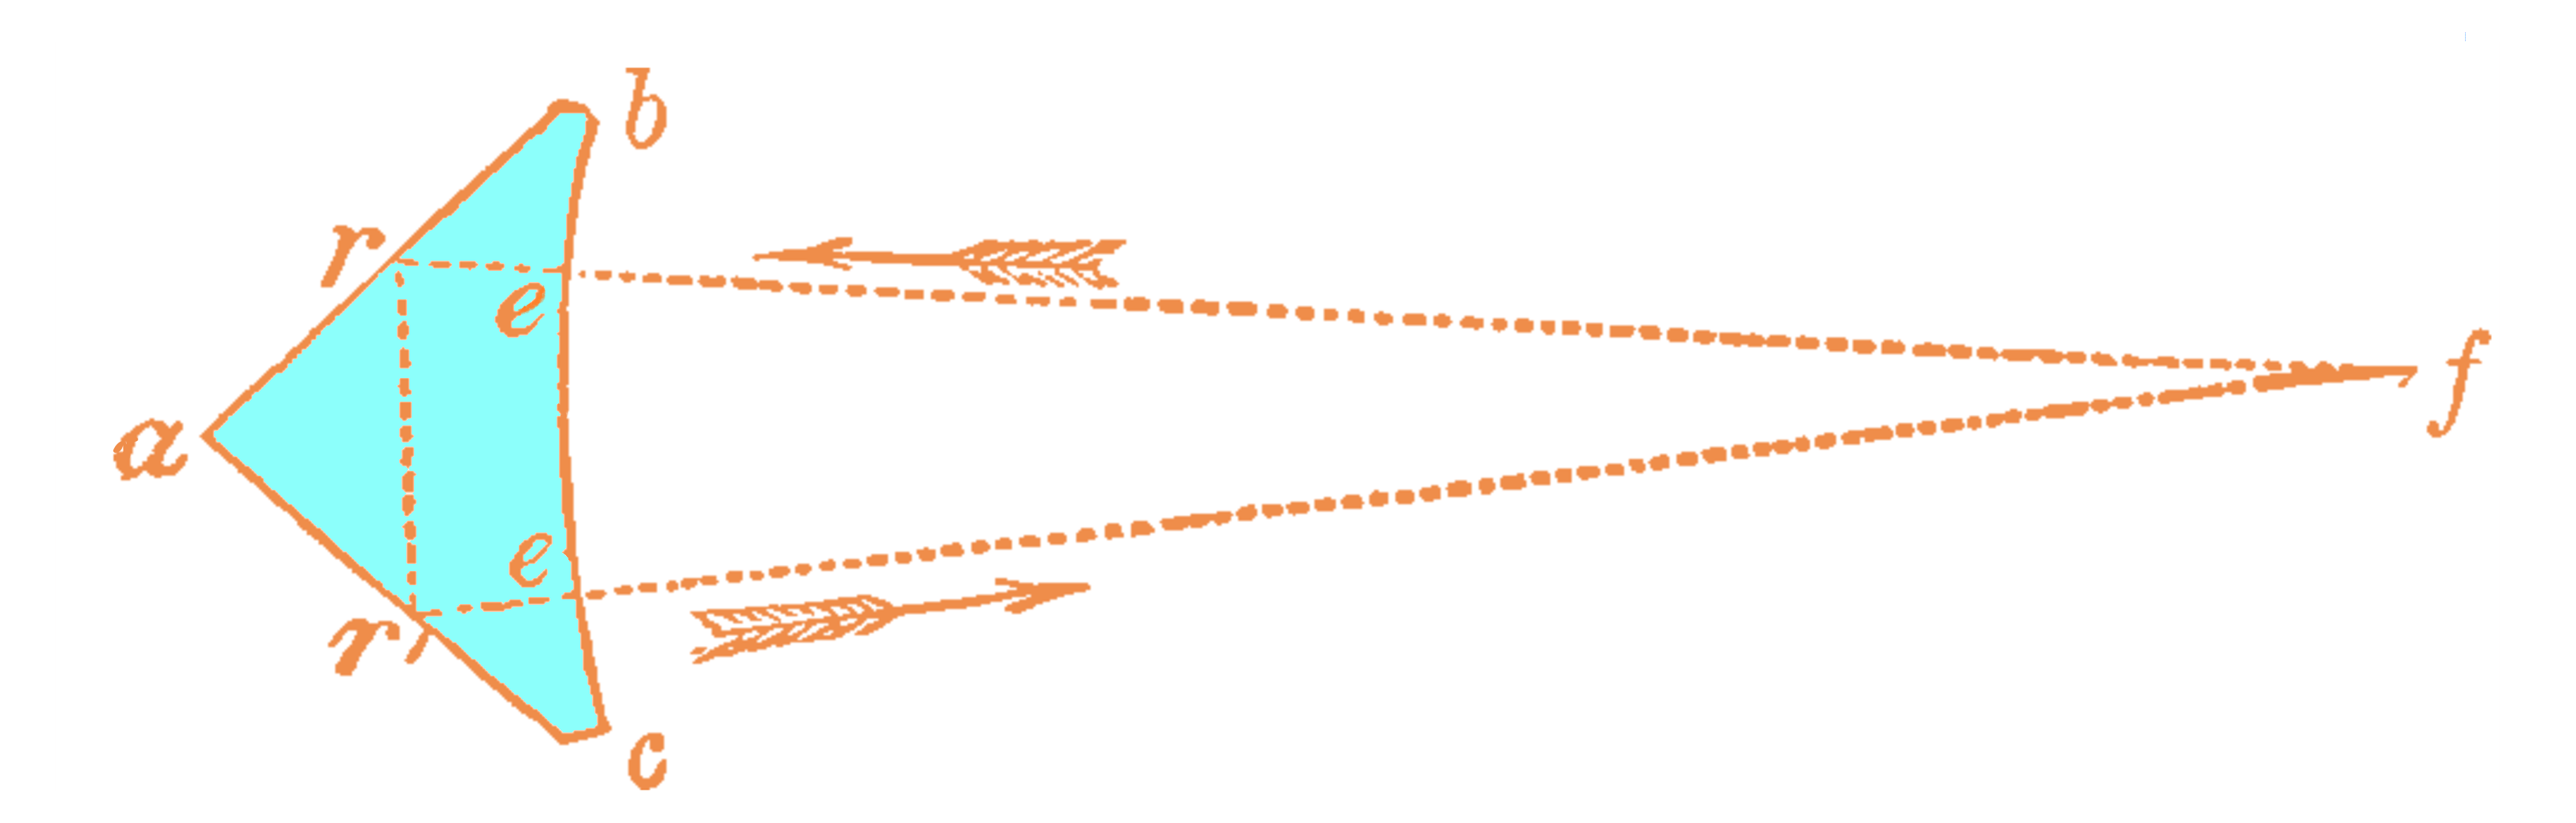
\includegraphics[width= 1\linewidth]{12a}
		$b)$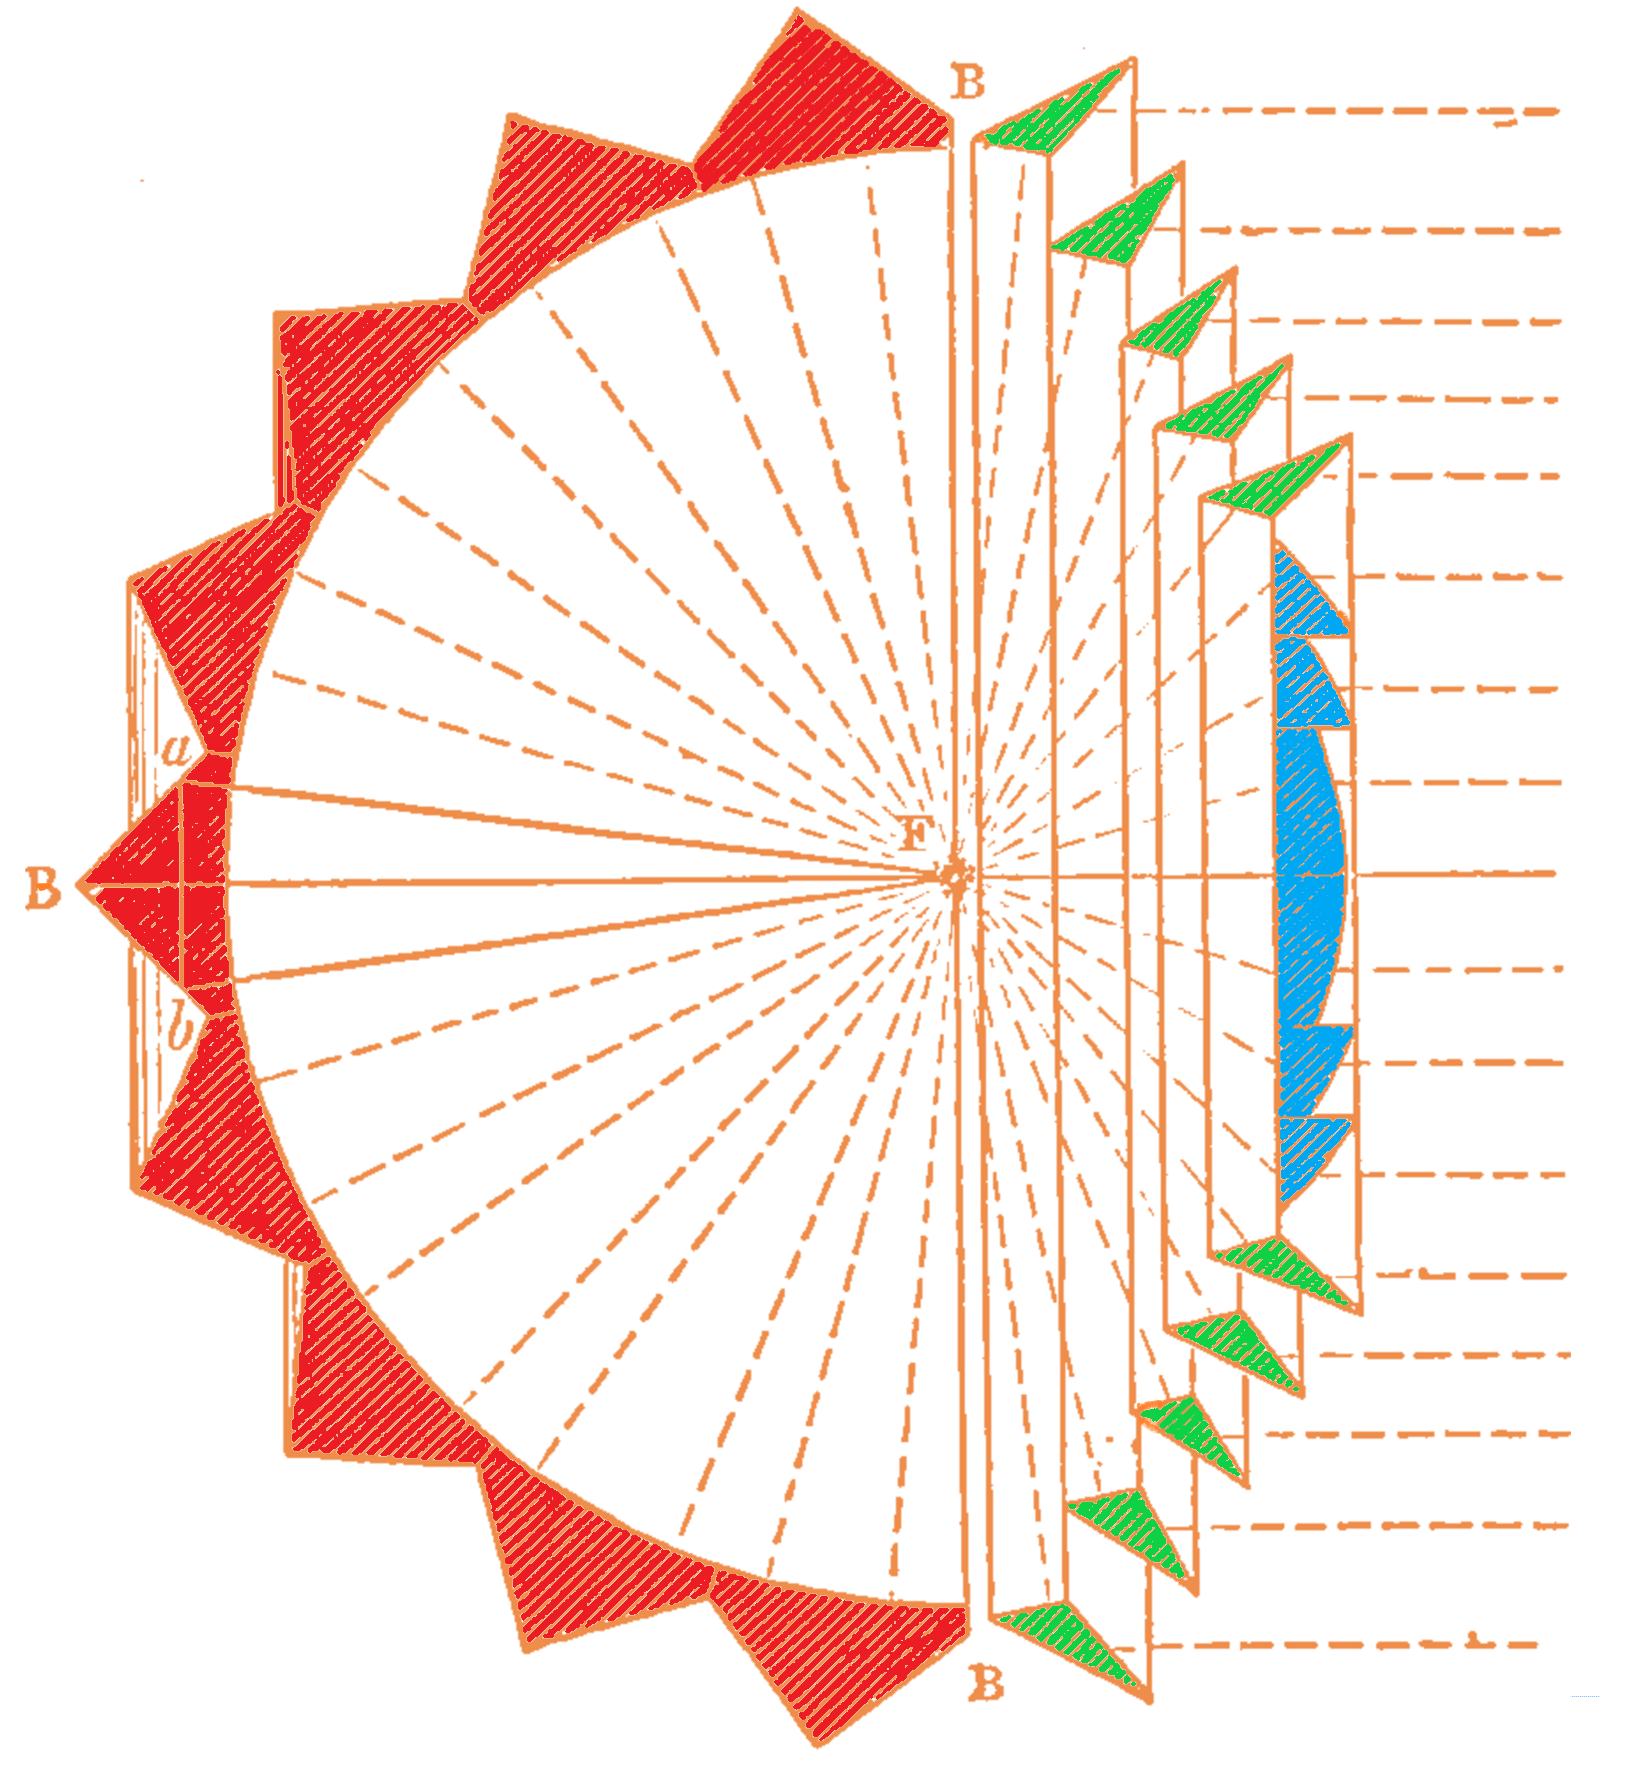
\includegraphics[width= 1\linewidth]{12b}
		\caption{\small\textit{\color{timhieukhoahoc}Hình $11$. $a)$ Lăng kính phản xạ kép. $b)$ Các lăng kính phản xạ kép tròn xoay (tô màu đỏ) được sử dụng thay cho mặt bán cầu kim loại ở phía sau nguồn sáng.}}
		\vspace*{-10pt}
	\end{figure}
	Một đột phá khác của Stevenson là việc sử dụng các lăng kính holophote trong hệ quang học quay cho hải đăng. Hệ thống đầu tiên dạng này được lắp đặt tại hải đăng North Ronaldsay ở Scotland. Trong khi phần giữa vẫn giữ nguyên cấu tạo có thiết diện đa giác đều với các tấm chứa thấu kính Fresnel, toàn bộ phần trên và phần dưới đều sử dụng thấu kính holophote để tạo chùm song song tương ứng với từng cạnh của đa giác (Hình $12$).
	\begin{figure}[H]
		\vspace*{-5pt}
		\centering
		\captionsetup{labelformat= empty, justification=centering}
		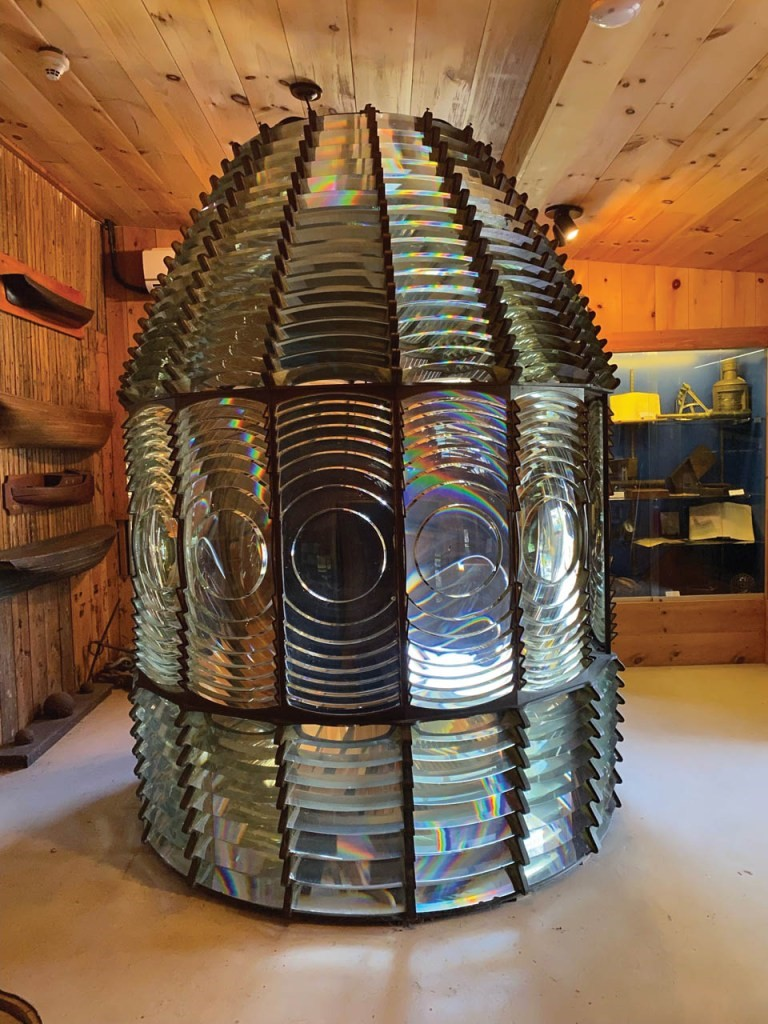
\includegraphics[height=0.4\linewidth]{13}
		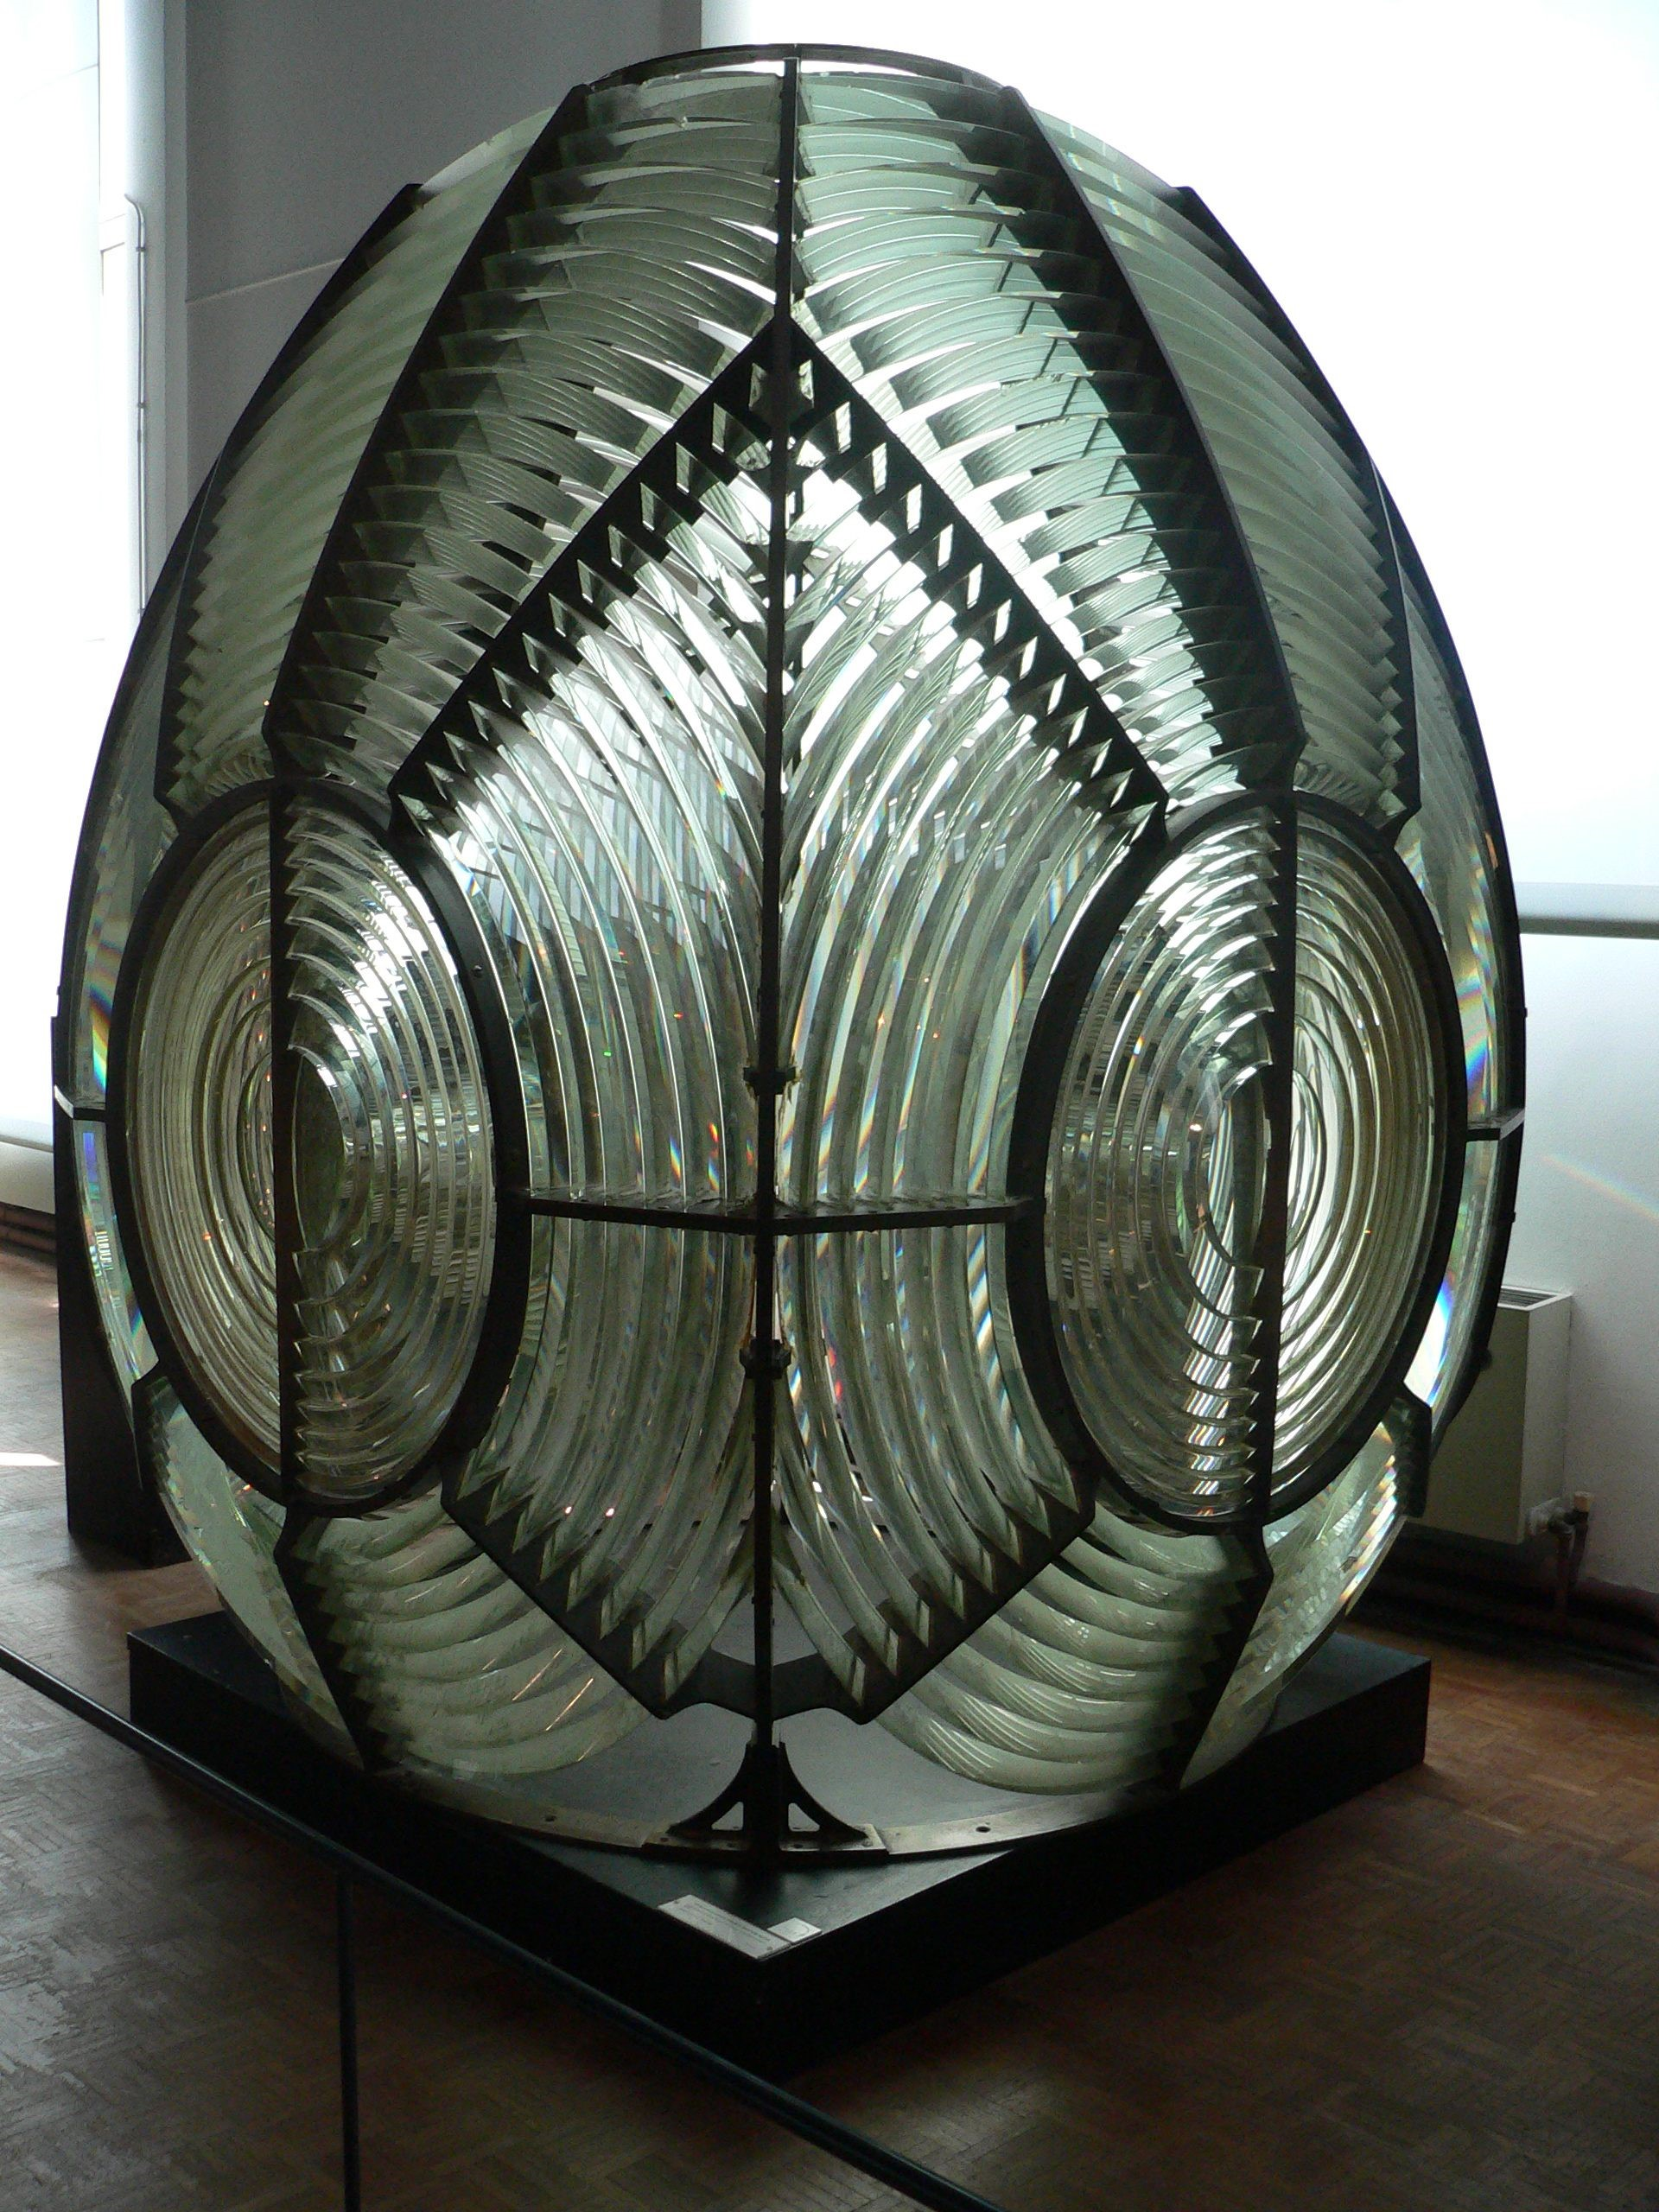
\includegraphics[height=0.4\linewidth]{13b}
		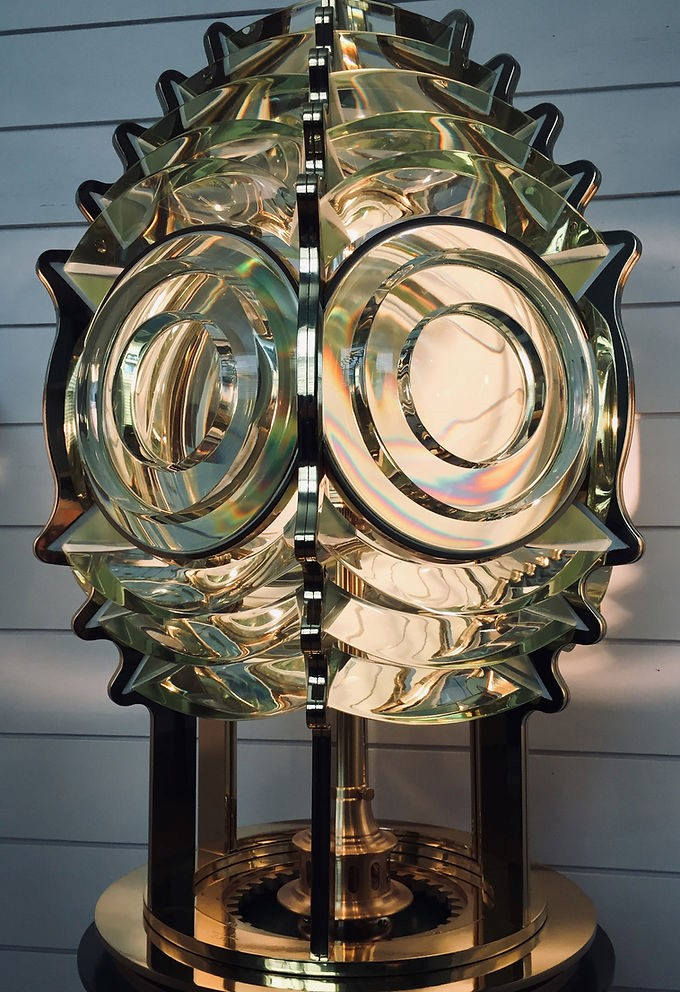
\includegraphics[height=0.4\linewidth]{13c}
		\caption{\small\textit{\color{timhieukhoahoc}Hình $12$. Một số hệ quang học quay cho hải đăng sử dụng thấu kính Fresnel và lăng kính holophote.}}
		\vspace*{-5pt}
	\end{figure}
	Một vấn đề quang học tiếp theo mà Stevenson giải quyết là việc làm thế nào phân bố ánh sáng tập trung vào một số hướng nhất định phục vụ yêu cầu thực tế. Ví dụ như với địa hình của eo biển, người ta muốn ánh sáng của hải đăng chiếu sáng nhiều hơn vào phần đường biển mà tàu thuyền đi lại thay vì chiếu đồng đều các phương. Các hệ thống quang học phức tạp gồm các lăng kính holophote xoay quanh thấu kính Fresnel, lăng kính phản xạ kép cùng các lăng kính dạng lăng trụ đứng được Stevenson thiết kế để giải quyết các nhu cầu thực tế này.
	\begin{figure}[H]
		\vspace*{-5pt}
		\centering
		\captionsetup{labelformat= empty, justification=centering}
		$a)$\includegraphics[width= 0.9\linewidth]{14a}
		$b)$\includegraphics[width= 0.9\linewidth]{14b}
		\caption{\small\textit{\color{timhieukhoahoc}Hình $13$. $a)$ Trong thực tế, có lúc người ta cần chiếu sáng tập trung vào một số phương nhất định. $b)$ Hệ thống có thêm các lăng kính dạng lăng trụ đứng (tô màu tím) để thực hiện việc trên của Thomas Stevenson.}}
		\vspace*{-10pt}
	\end{figure}
	$\pmb{3.}$ \textbf{\color{timhieukhoahoc}Thấu kính Fresnel trong các thiết bị hiện đại}
	\vskip 0.1cm
	Với sự ra đời của các nguồn sáng sử dụng điện từ đầu thế kỷ $20$, các hệ thống quang học trong hải đăng đã có thể được đơn giản hóa đi rất nhiều. Đồng thời, sự xuất hiện của các công nghệ định vị trên biển cũng làm giảm đi tầm quan trọng của hải đăng trong hàng hải. Tuy vậy, với ưu thế về kích thước và khối lượng nhỏ, thấu kính Fresnel vẫn được sử dụng rất phổ biến trong nhiều lĩnh vực của đời sống. 
	\vskip 0.1cm
	Thấu kính Fresnel xuất hiện trong nhiều ống kính cho máy ảnh cũng như các thiết bị quang học trong công nghiệp và nghiên cứu khoa học do nó có thể giúp giảm kích thước của hệ thống quang học. Tuy nhiên, do thấu kính này có thể gây ra nhiễu xạ ánh sáng, nó thường phải được kết hợp với nhiều cấu trúc quang học khác để đảm bảo chất lượng ảnh.
	\begin{figure}[H]
		\vspace*{-5pt}
		\centering
		\captionsetup{labelformat= empty, justification=centering}
		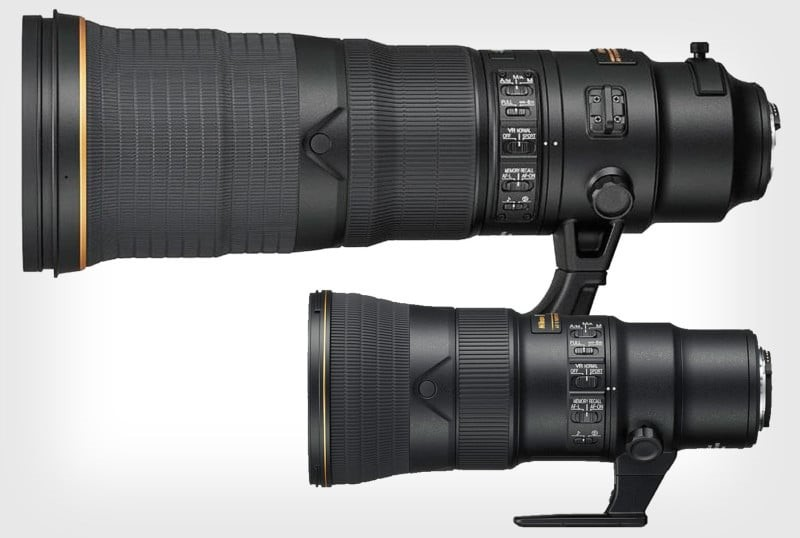
\includegraphics[width= 1\linewidth]{15}
		\caption{\small\textit{\color{timhieukhoahoc}Hình $14$. Hai ống kính chụp xa có cùng tiêu cự của cùng một hãng. Ống kính có sử dụng thấu kính Fresnel có kích thước nhỏ hơn nhiều, tuy nhiên lượng ánh sáng đến cảm biến sẽ nhỏ hơn.}}
		\vspace*{-10pt}
	\end{figure}
	Thấu kính Fresnel cũng được sử dụng trong một số thiết bị chiếu sáng như đèn chiếu cho sân khấu hay phòng chụp ảnh hoặc trong các máy chiếu.Trước khi màn hình tinh thể lỏng trở nên phổ biến, một số TV công nghệ CRT cũng sử dụng thấu kính Fresnel để giảm kích thước. Gần đây, một số thiết bị thực tại ảo đã dùng thấu kính Fresnel để phóng đại ảnh phía trước mắt người.
	\begin{figure}[H]
		\vspace*{-5pt}
		\centering
		\captionsetup{labelformat= empty, justification=centering}
		$a)$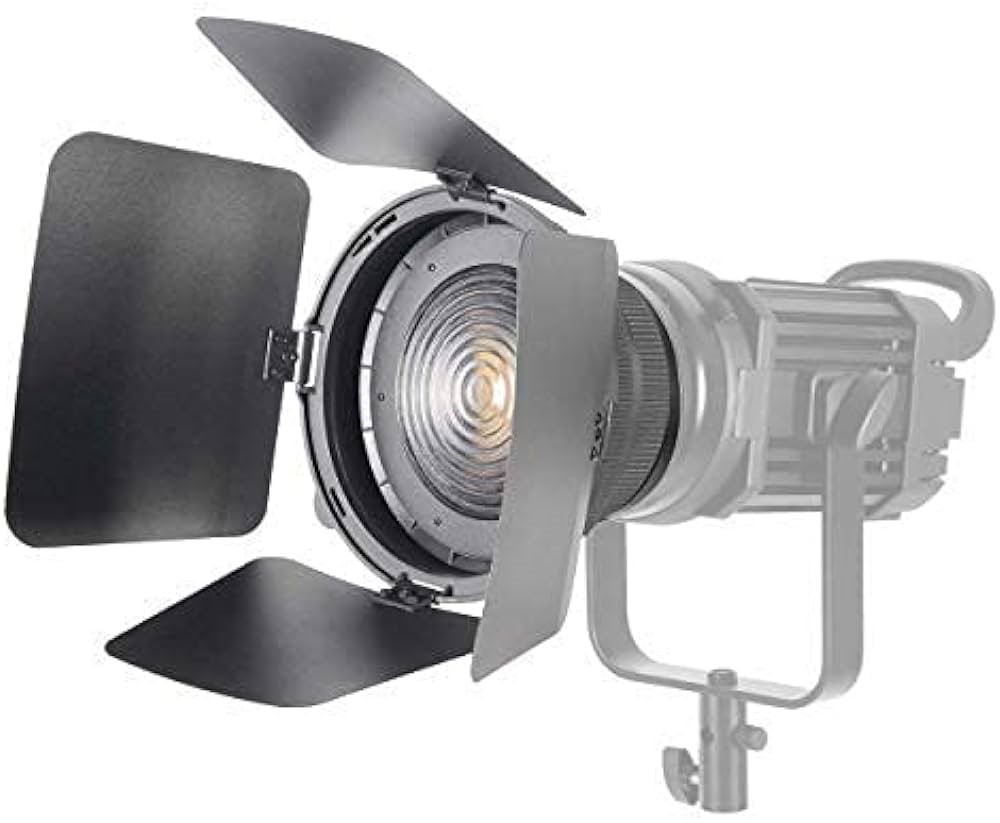
\includegraphics[width= 0.4\linewidth]{16a}
		$b)$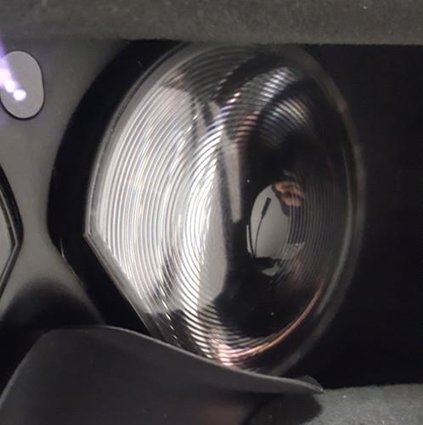
\includegraphics[width= 0.4\linewidth]{16b}
		\caption{\small\textit{\color{timhieukhoahoc}Hình $15$. Thấu kính Fresnel trong $a)$ đèn chiếu sân khấu và $b)$ Thiết bị thực tế ảo.}}
		\vspace*{-10pt}
	\end{figure}
	Do đặc tính nhỏ gọn, thấu kính Fresnel cũng xuất hiện ở các thiết bị cần kích thước nhỏ gọn như cảm biến hồng ngoại chống trộm hay thiết bị đọc mã vạch. Các thấu kính này có thể được làm bằng nhựa hoặc các dạng tấm mỏng tùy theo công nghệ sản xuất và nhu cầu của thiết bị.
	\begin{figure}[H]
		\vspace*{-5pt}
		\centering
		\captionsetup{labelformat= empty, justification=centering}
		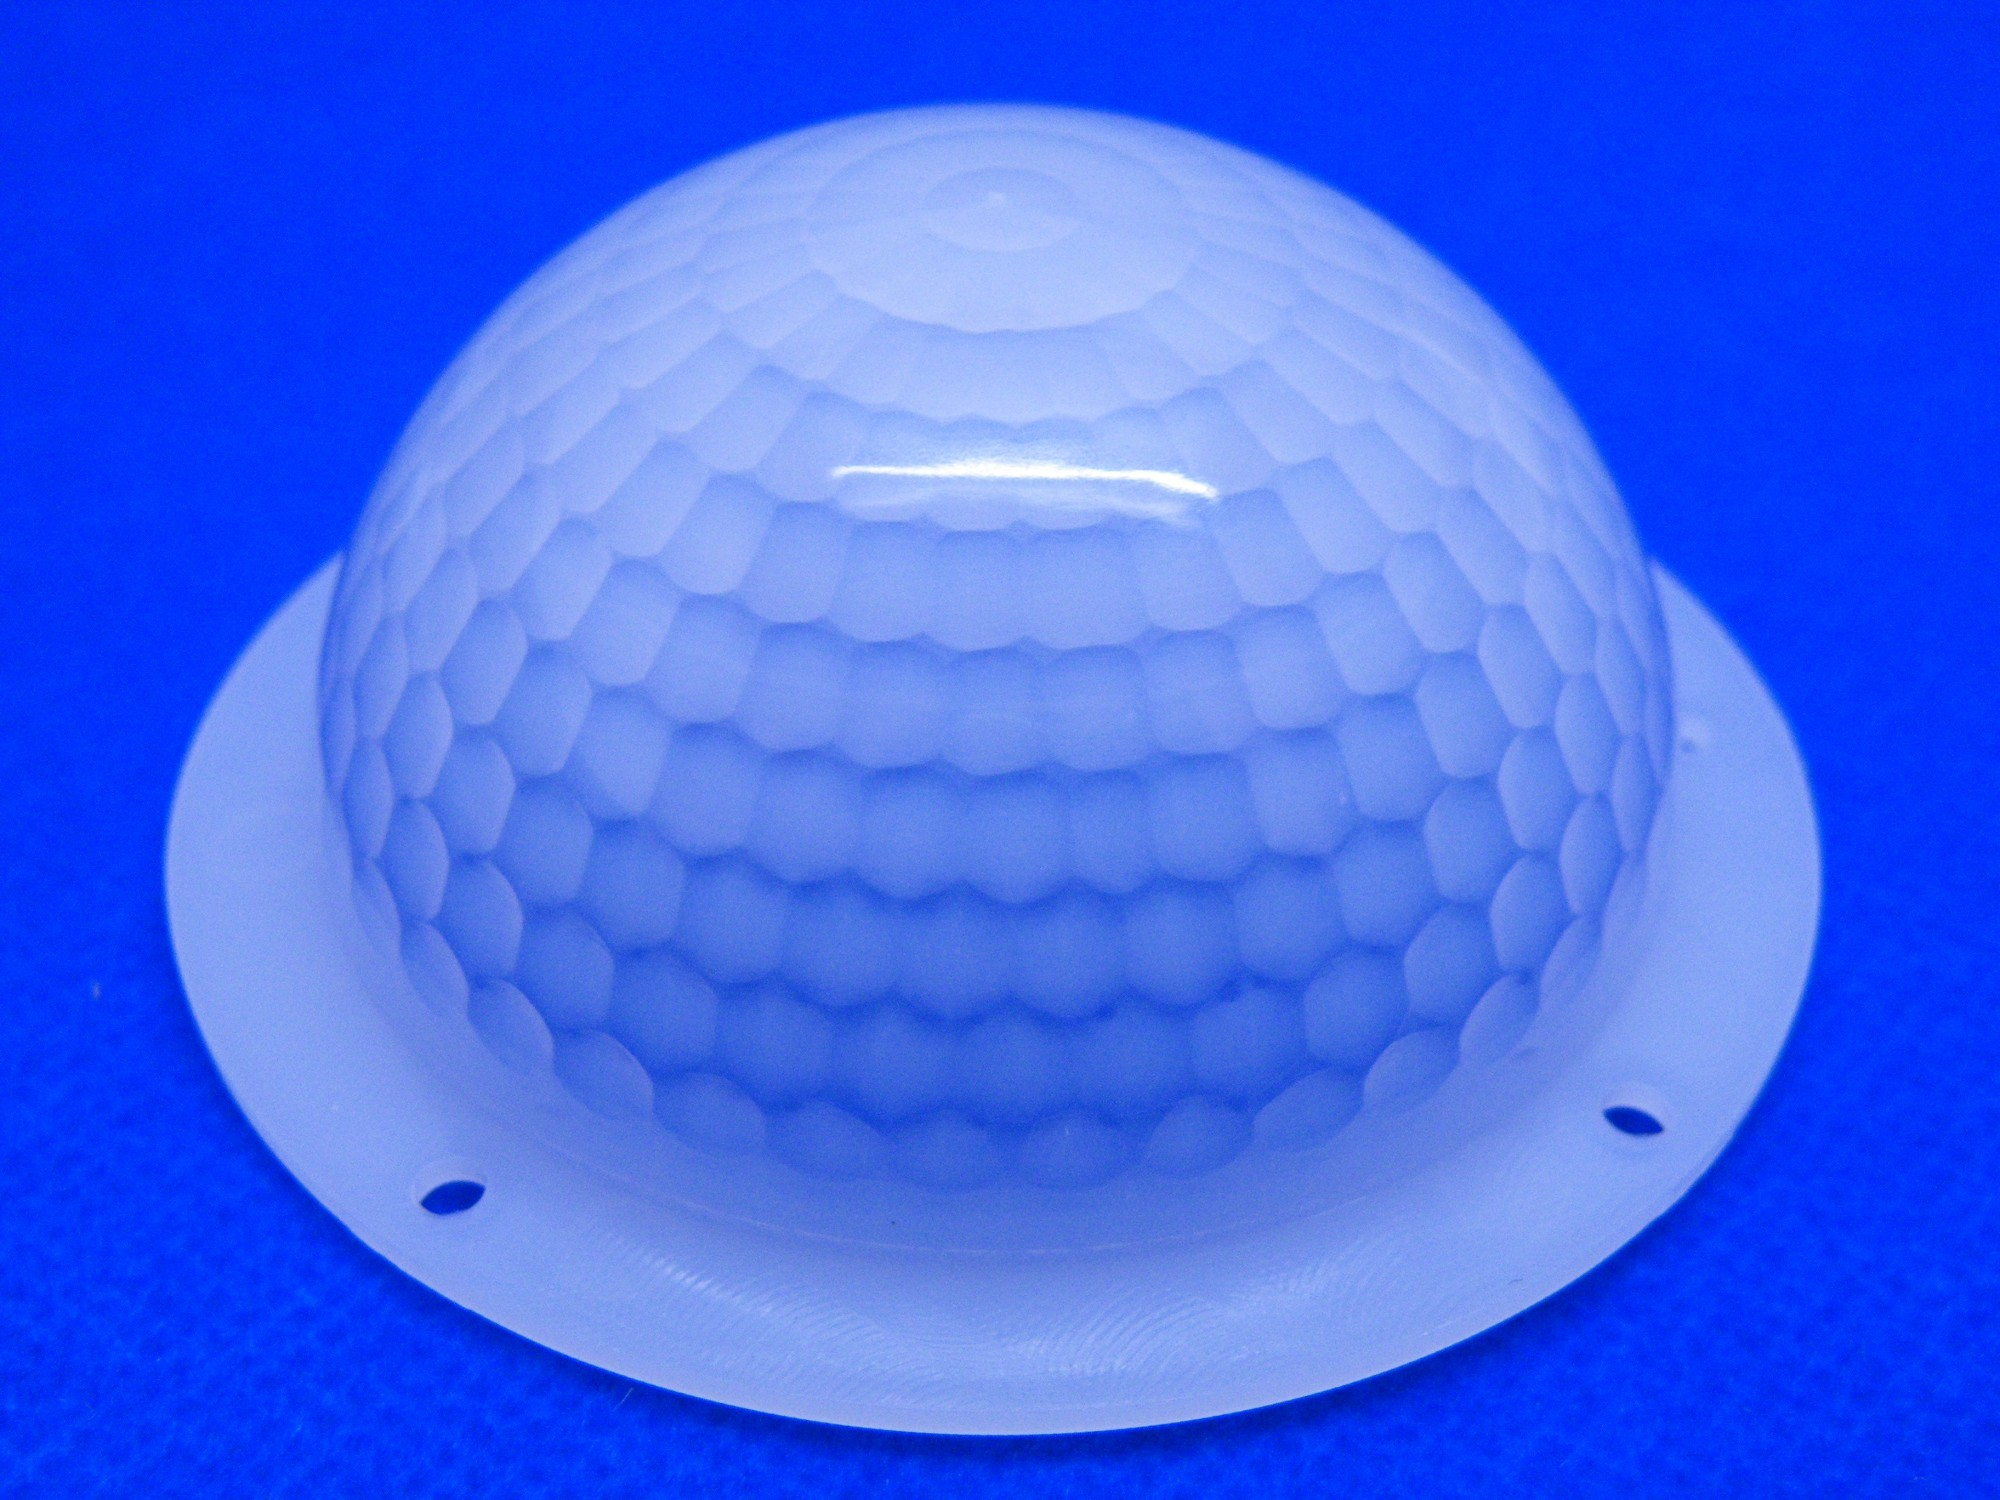
\includegraphics[width= 0.7\linewidth]{17}
		\caption{\small\textit{\color{timhieukhoahoc}Hình $16$. Thấu kính Fresnel trong thiết bị cảm biến hồng ngoại.}}
		\vspace*{-10pt}
	\end{figure}
	Trong giao thông, nhiều đèn tín hiệu được gắn thấu kính Fresnel để hướng ánh sáng đến vùng có phương tiện di chuyển, giúp dễ quan sát hơn. Nhiều loại đèn pha của ô tô cũng được lắp các thấu kính Fresnel để tạo chùm sáng song song. Các thấu kính Fresnel mỏng cũng có thể được dán ở cửa kính của các xe tải, giúp người lái xe quan sát được những vị trị sát với đầu xe. Thấu kính loại này cũng có thể được dán ở kính trước của các xe hơi, giúp người lái quan sát được đèn tín hiệu giao thông dù tầm nhìn bị khuất.
	\begin{figure}[H]
		\vspace*{-5pt}
		\centering
		\captionsetup{labelformat= empty, justification=centering}
		$a)$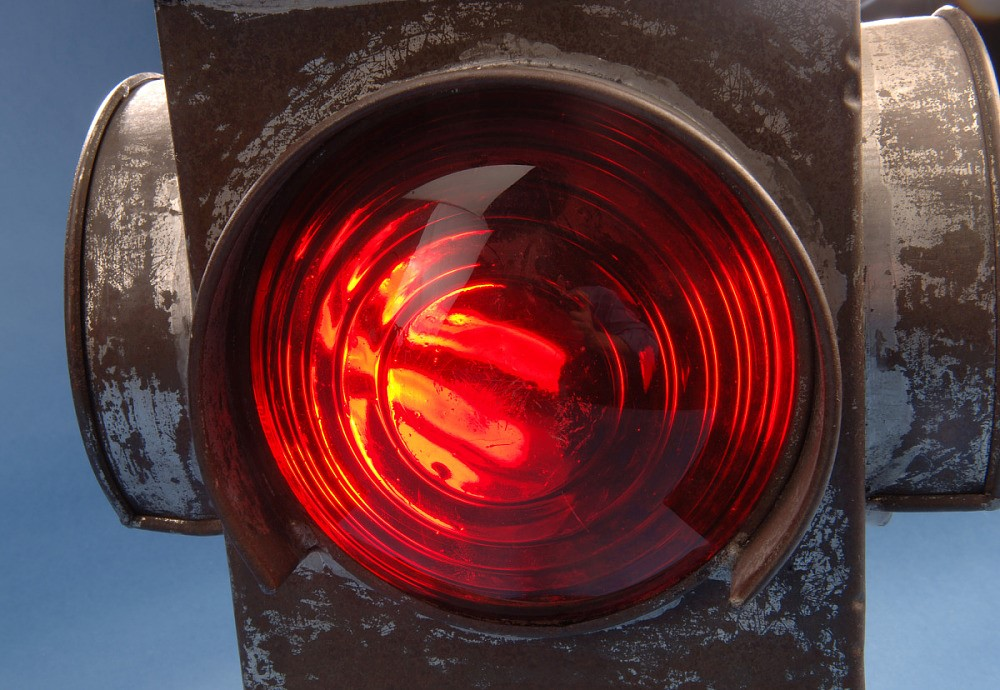
\includegraphics[height= 0.3\linewidth]{18a}
		$b)$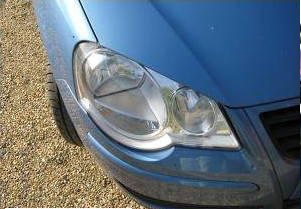
\includegraphics[height= 0.3\linewidth]{18b}
		
		$c)$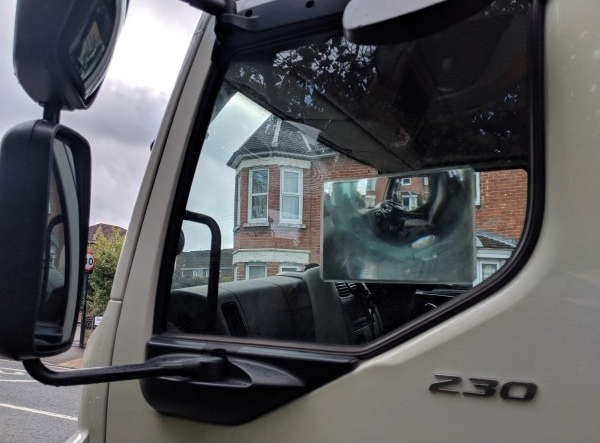
\includegraphics[height= 0.36\linewidth]{18c}
		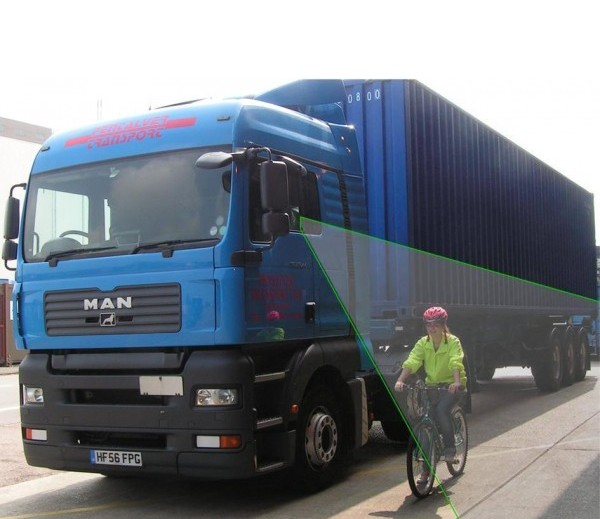
\includegraphics[height= 0.365\linewidth]{18d}
		\caption{\small\textit{\color{timhieukhoahoc}Hình $17$. $a)$ Thấu kính Fresnel của đèn tín hiệu. $b)$ Một số đèn pha ô tô cũng sử dụng thấu kính Fresnel. $c)$ Thấu kính Fresnel dạng miếng dán giúp xe tải quan sát điểm mù.}}
		\vspace*{-5pt}
	\end{figure}
	Giống như Buffon đã dự đoán, thấu kính Fresnel ngày nay còn được sử dụng để hội tụ ánh sáng. Khi lắp đặt các pin mặt trời, người ta có thể lắp thêm các thấu kính Fresnel nhằm tăng cường độ sáng tới các tấm pin. 
	\begin{figure}[H]
		\vspace*{-5pt}
		\centering
		\captionsetup{labelformat= empty, justification=centering}
		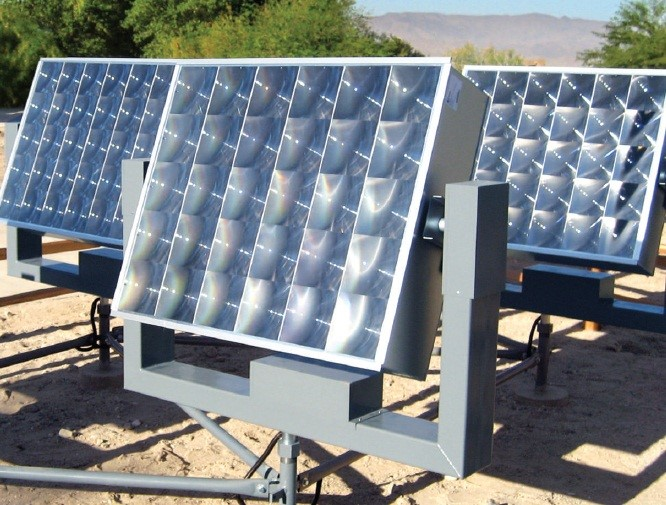
\includegraphics[width= 1\linewidth]{19}
		\caption{\small\textit{\color{timhieukhoahoc}Hình $18$. Thấu kính Fresnel hội tụ ánh sáng cho tấm pin mặt trời.}}
		\vspace*{-10pt}
	\end{figure}
	$\pmb{4.}$ \textbf{\color{timhieukhoahoc}Lời kết}
	\vskip 0.1cm
	Tuy Fresnel mất chỉ vài năm sau khi cho ra đời thấu kính mang tên ông, những người đi sau vẫn liên tục hoàn thiện các ứng dụng của nó, vào cả những lĩnh vực mà bản thân Fresnel có lẽ cũng sẽ cảm thấy ngạc nhiên. Không chỉ đảm bảo an toàn hàng hải cho rất nhiều con tàu của thế kỷ $19$, thấu kính Fresnel vẫn được sử dụng một cách đa dạng trong các thiết bị phục vụ đời sống nhờ sự đóng góp của các thế hệ nhà khoa học và kỹ sư nối tiếp nhau. Thấu kính Fresnel cũng là một chủ đề thú vị khi giảng dạy về quang học cho học sinh phổ thông. 
	\vskip 0.1cm
	\textbf{\color{timhieukhoahoc}Tài liệu tham khảo}
	\vskip 0.1cm
	[$1$] Basdevant, J.--L. ($2019$). Famous optician: Augustin Fresnel and the wave theory of light. \textit{Photoniques}, $18-22$. \url{https://doi.org/10.1051/photon/2019s418}
	\vskip 0.1cm
	[$2$] Elton, J. ($2009$). A Light to Lighten our Darkness: Lighthouse Optics and the Later Development of Fresnel's Revolutionary Refracting Lens $1780-1900$. \textit{Int. J. For the History of Eng. $\&$ Tech.}, $79(2)$, $183-244$.
	 \url{https://doi.org/10.1179/175812109x449612}
\end{multicols}